%----------------------------------------------------------------------------------------
%                   Galway-Mayo Institute of Technology (GMIT)
%                Department of Computer Science and Applied Physics
%
%                      *** Latex template for dissertations ***
%----------------------------------------------------------------------------------------

\documentclass[openany]{report}

\usepackage{graphicx} % Required for the inclusion of images
\usepackage[numbers]{natbib} % Required to change bibliography style to APA
\usepackage{amsmath} % Required for some math elements 
\usepackage{makecell}
\usepackage[english]{babel}
\usepackage{eurosym}
\usepackage{tabularx}
\usepackage{hyperref}
\usepackage[backend=biber]{biblatex}
\usepackage{tabularx}
\usepackage{pbox}
\usepackage{listings}
\usepackage[utf8]{inputenc}
\usepackage{hyperref}
\usepackage{color}
\usepackage{eurosym}
\usepackage{minted}
\usepackage[super]{nth}
\setlength\parindent{0pt} % Removes all indentation from paragraphs
\addbibresource{references.bib}
\newcommand*{\customTitle}{\begingroup % Create the command for including the title page in the document
\centering % Center all text
\vspace*{\baselineskip} % White space at the top of the page

\rule{\textwidth}{1.6pt}\vspace*{-\baselineskip}\vspace*{2pt} % Thick horizontal line
\rule{\textwidth}{0.4pt}\\[\baselineskip] % Thin horizontal line

%----------------------------------------------------------------------------------------
%	1) Change Dissertation Title
%----------------------------------------------------------------------------------------
{\Large E-Commerce Mobile Application   \\[2ex]}\\[0.2\baselineskip] % Title
%----------------------------------------------------------------------------------------


\rule{\textwidth}{0.4pt}\vspace*{-\baselineskip}\vspace{3.2pt} % Thin horizontal line
\rule{\textwidth}{1.6pt}\\[\baselineskip] % Thick horizontal line
\scshape % Small caps \\[\baselineskip] % Tagline(s) or further description
\Large \textbf{Final Year Project}\\
\textbf{B.Sc.(Hons) in Software Development}\par % Location and year
\normalsize
\vspace*{2\baselineskip} % Whitespace between location/year and editors


%----------------------------------------------------------------------------------------
%	2) Change Student Name(s)
%----------------------------------------------------------------------------------------
{by \\ Darren Regan  \par} % Editor list
%----------------------------------------------------------------------------------------


\vspace*{2\baselineskip} % Whitespace between location/year and editors
\vfill % Whitespace between editor names and publisher logo
{\scshape \today} \\[0.3\baselineskip] % Year published
%----------------------------------------------------------------------------------------


%----------------------------------------------------------------------------------------
%	3) Change Supervisor
%----------------------------------------------------------------------------------------

{\textbf{Advised by Martin Hynes}}\par % Supervisor

{Department of Computer Science and Applied Physics Galway-Mayo Institute of Technology (GMIT)}\par % Department
%----------------------------------------------------------------------------------------


\endgroup}
\begin{document} 
\pagenumbering{gobble}
\begin{figure}
\begin{center}

\includegraphics[width=8cm,height=3.3cm,keepaspectratio]{Images/gmit-logo.jpg}
\end{center}
\end{figure}
\customTitle
\tableofcontents
\listoffigures
\pagenumbering{arabic} 



%----------------------------------------------------------------------------------------
%	4) Change Chapters
%      Write each chapter in a separate TEX file and include here
%----------------------------------------------------------------------------------------

\chapter{Introduction}
My project is a Native Android E-Commerce Application built in Android Studio using Kotlin/Java programming languages. The general concept of my application is to create a e-commerce app that mirrors Amazon or Alibaba.

A specific goal of this project was to learn how native development differs from hybrid development(Xamarin, Ionic, React Native etc). Hybrid development was a topic that had multiple course projects, but i never got to experience building a project based on native development in Android or iOS.
\newline 

A focus i made on my application is integrating different technologies such as Firebase, Picasso and Retrofit. Using these technologies made certain aspects of my application easier to implement. For example Picasso which is a image downloading and caching library can manage many aspects of image processing in an android environment such as handling ImageView recycling, complex image transformations with minimal memory use and automatic memory and disk caching which all have a heavy amount of coding involved to be implemented manually. \newline

Firebase is another technology i use which has a great number of features and products such as Cloud Firestore which stores and syncs data between users and devices - at global scale - using a cloud-hosted, NoSQL database.

Authentication to manage users in a secure way by offering authentication through email, password and third-party providers like GitHub, Google, Facebook and Twitter.

Realtime Database which is an efficient, low-latency solution for mobile apps that require synced states across clients in realtime.
\newline 



\newpage
\subsection{Objectives for project}

\textbf {Use a new programming language and framework} 

One of the objectives i had set for this project is to use a new language and framework, i made the choice of android and kotlin as it met all my objectives for my project. The main goal of my project was to build a native mobile application and compare it to hybrid applications that i have built throughout my course.\newline


\textbf {Create a Native Mobile Application} 
\newline

\textbf {Use new and useful technologies}
ss \newline
\textbf {Include social Media Integration}
ss \newline

\textbf {Create a Native Mobile Application} \newline

\newpage

\subsection{Sections}

\textbf {Methodology}
After setting objectives for my project, i set out to make a plan for development using Kanban boards. I used an agile approach for my development setting specific goals for each week. Validation and Testing was done using Junit.
\newline


\textbf {Technology Review}
In this section i explain the Technologies used in my project, technologies such as Firebase, Kotlin, Android Studio are explained in great detail. I will also review programming in android with kotlin compared to my experience through out my four years in college. Comparisons such as Native development vs Hybrid development, use cases for different programming languages, language features such as more use of lambda expressions and more Kotlin features that make it a great alternative to java for android development.
\newline


\textbf {System Design}
In this section i provided an explanation of the overall system architecture using UML class, sequence and interaction diagrams as well as screenshots of UI components such as how each view is formed with ImageView, TextBox etc. \newline

\textbf {System Evaluation}
  In this section i evaluate my project against the objectives i set out. \newline

\textbf {Conclusion}

 In my conclusion i evaluate my overall goals for my project and list outcomes of the project. I go over discoveries made, what I've learned and what i can improve on in the future \newline

\textbf {Github Repository} \url{https://github.com/DarrenRegan/Final-Year-Project}
\newline

    My GitHub Repository contains my Dissertation, APK file which are both available for download with a click of a button at the top of the README. 
\begin{itemize}
     \item The README contains a quick explanation of the project as well as an installation guide, Devices used in testing as well as resources used along with links to research material.
         
     \item The code for my project is located at Final-Year-Project/app/src/main/
     Java folder contains the code for activities and models
     
    \item Res folder contains the code for UI elements of the project, \newline              main/res/layout contains XML for all activities
\end{itemize}



\begin{figure}[h!]
	\caption{The image caption should be succinct but descriptive.}
	\label{image:myImageName}
	\centering
	
\includegraphics[width=0.9\textwidth]{Images/gmit-building.png}
\end{figure}	
\chapter{Methodology}
This chapter covers the various methodologies that were implemented in this project, this includes Research methodologies, Software development methodologies, project management, supervisor meetings, developments tools, testing and source control.


An overview of methodologies used in this project; \textbf{Research methodologies} which includes Mixed Methods, Quantitative Research and Qualitative Research.
\textbf{Software development methodologies} which includes Agile Development, Continuous Delivery, Test Driven Development, Feature Driven Development, Extreme Programming etc.
\textbf{Project management} which includes GitHub Kanban board and supervisor meetings.
\textbf{Development tools} Android studio, Firebase.
\textbf{Source Control} GitHub, Overleaf, Badge/Shield

\newpage

\section{Research Methodology}
The research methodology that was used in this project was a Mixed Methods 
Research methodology, using a mix of both Qualitative Research and Quantitative 
Research. Qualitative research approaches are employed across many academic 
disciplines and is useful at an individual level. Qualitative data collection
methods vary using unstructured or semi-structured techniques.

\medskip
Various data collection tools were used for gathering data such as

\section{Software Development Methodology}
\begin{center}
    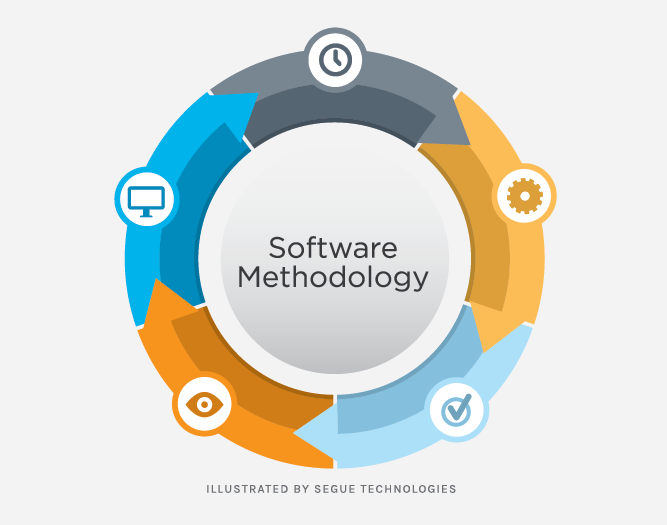
\includegraphics[width=5cm,keepaspectratio]{Images/Software_Method.png}
    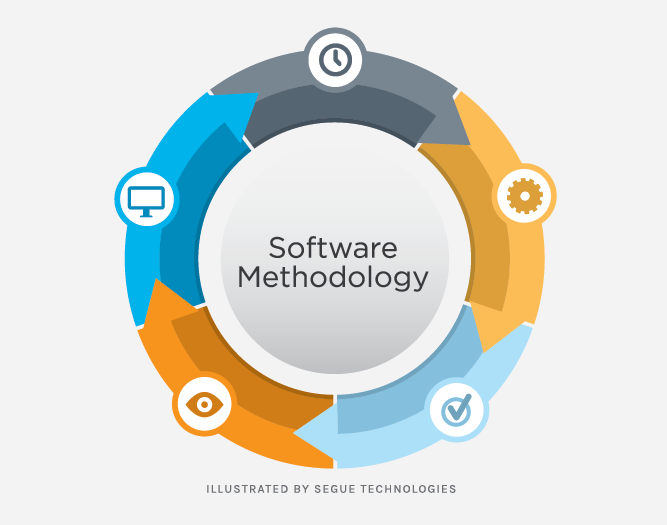
\includegraphics[width=5cm,keepaspectratio]{Images/Software_Method.png}
\end{center}

\par
\par
\medskip


Explain Agile Development, Continuous Delivery, Test Driven Development, Feature Driven Development, Extreme Programming etc.
How i implemented them in my project

\section{Project management}
Explain GitHub Kanban board and supervisor meetings. How i used both to improve my project

\section{Development tools}
Explain Android Studio, Firebase. Compare Android studio to Intellij

\section{Source Control}
Explain GitHub, Overleaf, Badge/Shield. 

\chapter{Technology Review}
This chapter discusses the different technologies used in throughout the
project. It discusses the the advantages and disadvantages of each technology 
and why certain technologies were used over others. It also discusses hybrid applications compared to native applications, advantages, disadvantages, uses at different business structures and other topics.

\section{Overview}
This project is a Native android app built with Kotlin in Android Studio, Firebase is used for the database, statistics, verification etc.

Topics:
\begin{itemize}
    \item Kotlin/Java comparison
    \item Fire-base
    \item Picasso
    \item Android Studio/IntelliJ
    \item Native Applications
    \item Hybrid Applications
    \item Hybrid vs Native comparison 
\end{itemize}
\newpage

\section{Main Technologies}
This section will discuss the main technologies currently in use in the android application.
%----------------------------------------------------------------------------------------
% KOTLIN
%----------------------------------------------------------------------------------------
\subsection{Kotlin}
\par
\medskip
\begin{center}
    
\includegraphics[width=12cm,height=12cm,keepaspectratio]{Images/Kotlin.png}
\end{center}
Kotlin is a cross-platform, statically typed, general-purpose programming language with type inference. Kotlin is designed to inter-operate fully with Java, and the JVM version of its standard library depends on the Java Class Library, but type inference allows its syntax to be more concise. Kotlin mainly targets the JVM, but also compiles to JavaScript or native code (via LLVM). Language development costs are borne by JetBrains, while the Kotlin Foundation protects the Kotlin trademark.

Kotlin is the preferred language for Android app developers as of May 2019, since the release of Android Studio 3.0 in October 2017, Kotlin has been included as an alternative to the standard Java compiler. The Android Kotlin compiler targets Java 6 by default, and lets programmers choose between Java 8 to 14 for optimization purposes.

Kotlin originated at JetBrains, which is the company behind IntelliJ IDEA. Kotlin has been open source since 2012 and has a large team of full-time developers working on it, there is also the \hyperlink{https://github.com/JetBrains/kotlin}{Kotlin project of GitHub} which has more than 370 contributors.

\newpage

\subsubsection{Advantages}
Kotlin has many advantages, many are quite serious improvements in readability and workflow which was noticeable when creating my project

\begin{itemize}
    \item \textbf{Less code combined with greater readability} - Spend less time writing code and working to understand the code of others.
    \item \textbf{Mature language and environment} - Kotlin has developed continuously over the years not only as a language but as a whole ecosystem with very robust tooling. Its seamless integration with Android Studio, makes it actively used by companies to develop Android applications.
    \item \textbf{Kotlin support of Android Jetpack and other libraries} - \hyperlink{https://developer.android.com/kotlin/ktx}{KTX extensions} adds kotlin language features, such as coroutines, extension functions, lambdas, and named parameters, to existing Android libraries.
    \item \textbf{Interoperability with Java} - You can use Kotlin along with the Java programming language in your applications without needing to migrate all your code to Kotlin. 
    \item \textbf{Support for multi-platform development} - You can use Kotlin for developing not only Android but also iOS, back-end, and web applications by sharing the common code among the platforms.
    \item \textbf{Code safety} - Less code and better readability lead to fewer errors. The Kotlin compiler detects the remaining errors, making the code safe. 
    \item \textbf{Easy to Learn} - Kotlin is very easy to learn, especially for any Java experienced developers. 
    \item \textbf{Large community} - Kotlin a great support and many contributions from the community, which is growing all over the world. According to Google, over 60\% of the top 100 apps on the Google Play Store use Kotlin. Many startups and Fortune 500 companies have already developed Android applications using Kotlin and more and more companies are prioritizing Kotlin Native application development over other options due to the robust toolkit and optimizations that make your applications the best that they can be. 
\end{itemize}

\newpage

\subsubsection{Disadvantages}

\begin{itemize}
    \item \textbf{Shift from Java to Kotlin} - Kotlin is an amazing programming language and there is a reason why leading lead companies have started using kotlin, but at their core their two different languages. Developers won't be able to quickly shift from one to another without taking time to learn Kotlin. Therefore company's have to consider different approaches to Android app development as additional expenses are required on training a team of developers. 
    \item \textbf{Hard to find experienced developers} - There is a high demand for specialists in Kotlin as Google made it the preferred language for Android development in 2019, but there is still a very large amount of Java programmers on the market compared to Kotlin developers. This means on average the Kotlin developers may be younger meaning less senior developers available for hire. This is quite a large disadvantage, but will quickly fade away as many leading tech companies have switched which creates a ripple effect down the chain of companies.
    \item \textbf{Limited learning resources} - Although the number of Android app developers who use Kotlin instead of Java increase everyday, there is still a limited number of resources in the market compared to Java. Many College courses will teach Java over Kotlin as both are so similar, meaning most Kotlin developers come from a background in Java and learn to code in Kotlin themselves.
\end{itemize}

\newpage
\subsubsection{Kotlin Syntax}
Kotlin syntax is familiar to any programmer that is from a OOP domain and be be more or less understood from the get-go. There are differences from Java such as primary and secondary constructors, val \& var variable declarations and more.
\newline

\textbf{Below you can see the basic structure of a class in kotlin}
\begin{lstlisting}
class Foo {

    val b: String = "b"     // val means unmodifiable
    var i: Int = 0          // var means modifiable

    fun hello() {
        val str = "Hello"
        print("$str World")
    }

    fun sum(x: Int, y: Int): Int {
        return x + y
    }

    fun maxOf(a: Float, b: Float) = if (a > b) a else b

}
\end{lstlisting}

\textbf{String Interpolation} - A smarter and more readable version of Java's String.format() that is built into the language
\begin{lstlisting}
val x = 5
val y = 10
print("sum of $x and $y is ${x + y}")  // sum of 5 and 10 is 15
\end{lstlisting}

\textbf{Type Inference} - Kotlin will infer your types wherever you feel it will improve readability
\begin{lstlisting}
val a = "abc"                         // type inferred to String
val b = 4                             // type inferred to Int

val c: Double = 0.7                   // type declared explicitly
val d: List<String> = ArrayList()     // type declared explicitly
\end{lstlisting}

\textbf{Smart Casts} - The Kotlin compiler tracks logic and auto-casts types if possible, which means you do not need to use instanceof checks followed by explicit casts
\begin{lstlisting}
if (obj is String) {
    print(obj.toUpperCase())     // obj is now known to be a String
}
\end{lstlisting}

\textbf{When Expression} - The switch case is replaced with the more readable and flexible when() expression
\begin{lstlisting}
when (x) {
    1 -> print("x is 1")
    2 -> print("x is 2")
    3, 4 -> print("x is 3 or 4")
    in 5..10 -> print("x is 5, 6, 7, 8, 9, or 10")
    else -> print("x is out of range")
}

// It also works as an expression or a statement
// with or without an argument
val res: Boolean = when {
    obj == null -> false
    obj is String -> true
    else -> throw IllegalStateException()
}
\end{lstlisting}

\textbf{Setter \& Getter behavior} - You can make custom set \& get behaviors that are added to public fields, which means getter \& setters won't bloat your code
\begin{lstlisting}
class Frame {
    var width: Int = 800
    var height: Int = 600

    val pixels: Int
        get() = width * height
}
\end{lstlisting}

\textbf{Data Classes} - We frequently create classes whose main purpose is to hold data. In such a class some standard functionality and utility functions are often mechanically derivable from the data. In kotlin, this is called a data class and is marked as data. Its a Plain Old Java Object so its complete with toString(), equals(), hashCode() and copy().
\begin{lstlisting}
data class Person(val name: String,
                  var email: String,
                  var age: Int)

val john = Person("John", "john@gmail.com", 112)
}
\end{lstlisting}

\subsection{Kotlin vs Java}
\par
\medskip
\begin{center}
    
\includegraphics[width=12cm,height=12cm,keepaspectratio]{Images/KotlinvJava.jpg}
\end{center}

blah..


\subsubsection{Advantages}
\begin{itemize}
    \item \textbf{Shift from Java to Kotlin} - Kotlin
    \item \textbf{Hard to find experienced developers} - asdas
    \item \textbf{Limited learning resources} - Although
\end{itemize}
\subsubsection{Disadvantages}
\begin{itemize}
    \item \textbf{Shift from Java to Kotlin} - Kotlin
    \item \textbf{Hard to find experienced developers} - asdas
    \item \textbf{Limited learning resources} - Although
\end{itemize}

\newpage

%----------------------------------------------------------------------------------------
% FIREBASE
%----------------------------------------------------------------------------------------
\subsection{Firebase}
\par
\medskip
\begin{center}
    
\includegraphics[width=12cm,height=12cm,keepaspectratio]{Images/firebase.png}
\end{center}

Firebase is Google's mobile and web application development platform that helps you build, improve, and grow your application. Firebase frees developers to focus on crafting excellent user experiences. You don't need to manage servers. You don't need to write APIs. Firebase is your server, your API and your database, everything is written generically so that you can modify everything to suit most needs. Firebase has a huge amount of features, real time databases, cloud storage, hosting, machine learning, authentication, statistics, analytics and more.\newline

Firebase products are setup in three different area's.
\begin{enumerate}
  \item \textbf{Build better apps}
  \item \textbf{Improve app quality}
  \item \textbf{Grow your business}
\end{enumerate}

\subsubsection{Build better apps} Firebase lets you build more powerful, secure and scalable apps, using world-class infrastructure. There are seven different products focused on building a better app. My project takes advantage of Authenication, Realtime Database and Cloud storage. Almost all of Firebase products are extremely useful and are worth mentioning as they could be implemented into the project at some point.
I will first summarize the products, and then go into further detail on the specific products i used in my project. How the code is implemented, why i used it etc.

\newpage
\subsubsection{Products for building better apps}
\begin{itemize}
    \item \textbf{Cloud Firestore} - Store and sync data between users and devices - at global scale - using a cloud-hosted, NOSQL database. Cloud Firestore gives you live synchronization and offline support along with efficient data queries. Its integration with other Firebase products enables you to build truly serverless apps.
    \item \textbf{ML Kit} - Bring powerful machine learning features to your mobile app whether you're new or experienced in ML. Get started easily by using our ready-to-use APIs for common mobile use cases, or import your own custom models which can be hosted and served to your apps by Firebase. ML Kit APIs can run on-device or in the cloud, depending on the functionality, and some give you both choices.
    \item \textbf{Cloud Functions} - Extend your app with custom backend code without needing to manage and scale your own servers. Functions can be triggered by events, which are emitted by Firebase products, Google Cloud services, or third parties, using webhook
    \item \textbf{Authentication} - Manage your users in a simple and secure way. Firebase Auth offers multiple methods to authenticate, including email and password, third-party providers like Google or Facebook, and using your existing account system directly. Build your own interface, or take advantage of our open source, fully customizable UI.
    \item \textbf{Hosting} - Simplify your web hosting with tools made specifically for modern web apps. When you upload your web assets, we automatically push them out to our global CDN and give them a free SSL certificate so your users get a secure, reliable, low-latency experience, no matter where they are.
    \item \textbf{Cloud Storage} - Store and share user-generated content like images, audio, and video with powerful, simple, and cost-effective object storage built for Google scale. The Firebase SDKs for Cloud Storage add Google security to file uploads and downloads for your Firebase apps, regardless of network quality.
    \item \textbf{Realtime Database} - Realtime Database is Firebase's original database. It's an efficient, low-latency solution for mobile apps that require synced states across clients in realtime. We recommend Cloud Firestore instead of Realtime Database for most developers starting a new project.
\end{itemize}

\newpage
\subsubsection{Improve app quality}
Firebase gives you insights into app performance and stability, so you can channel your resources effectively.
These products weren't used in the project, but are worth mentioning as they are quite valuable in a commercial development environment where app performance and crashing have a huge impact on user engagement and app performance on the Google Play Store.

\subsubsection{Products for improving app quality}
\begin{itemize}
    \item \textbf{Crashlytics} - Reduce your troubleshooting time by turning an avalanche of crashes into a manageable list of issues. Get clear, actionable insight into which issues to tackle first by seeing the user impact right in the Crashlytics dashboard. Realtime alerts will help you stay on top of stability even on the go. Crashlytics is the primary crash reporter for Firebase.
    \item \textbf{Performance Monitoring} - Diagnose app performance issues occurring on your users’ devices. Use traces to monitor the performance of specific parts of your app and see a summarized view in the Firebase console. Stay on top of your app’s start-up time and monitor HTTP requests without writing any code.
    \item \textbf{Test Lab} - Run automatic and customized tests for your app on virtual and physical devices hosted by Google. Use Firebase Test Lab throughout your development lifecycle to discover bugs and inconsistencies so that you can offer up a great experience on a wide variety of devices.
    \item \textbf{App Distribution} - Firebase App Distribution allows developers to send pre-release versions of their app to trusted testers from the console or using command line tools, as well as manage testers in one place.
\end{itemize}


\newpage
\subsubsection{Grow your business}
Firebase helps you grow to millions of users, simplifying user engagement and retention.

\subsubsection{Products for Growing your business}
\begin{itemize}
    \item \textbf{In-App Messaging} - Engage and nurture your active users with targeted and contextual messages that encourage them to complete meaningful actions within your app. You have the power to trigger messages based on user behavior and interests. You can also customize the design of in-app messages to fit your brand. In-App Messaging supports a variety of use cases and formats.
    \item \textbf{Google Analytics} - Analyze user attributions and behavior in a single dashboard to make informed decisions on your product roadmap. Gain realtime insights from reports, or export your raw event data to Google BigQuery for custom analysis.
    \item \textbf{Predictions} - Harness the power of Google’s machine learning to get insight into which segments of users are likely to churn or spend (or complete another conversion event). Use these smart predictive segments for targeting in other products like Remote Config, Cloud Messaging, and In-App Messaging.
    \item \textbf{A/B Testing} - Improve your app by running product and marketing experiments, without worrying about setting up the infrastructure to run A/B tests. Customize experiments to suit your goals. Test a variety of updates to your app, like message copy or new features. Then, only roll-out changes proven to move the needle on your key metrics.
    \item \textbf{Cloud Messaging} - Send messages and notifications to users across platforms—Android, iOS, and the web—for free. Messages can be sent to single devices, groups of devices, or specific topics or user segments. Firebase Cloud Messaging (FCM) scales to even the largest apps, delivering hundreds of billions of messages per day.
    \item \textbf{Remote Config} - Customize how your app renders for each user. Change the look and feel, roll out features gradually, run A/B tests, deliver customized content to certain users, or make other updates without deploying a new version—all from the Firebase console. Monitor the impact of your changes and make adjustments in a matter of minutes.
    \item \textbf{Dynamic Links} - Use Dynamic Links to deliver a customized user experience for iOS, Android, and the web. You can use them to power mobile web to drive native app conversions, user to user sharing, social and marketing campaigns, and more. Dynamic Links provides you with the attributions you need to better understand your mobile growth.
    
    
\end{itemize}



\subsubsection{Traditional Architecture vs. Serverless Architecture}
\begin{center}
    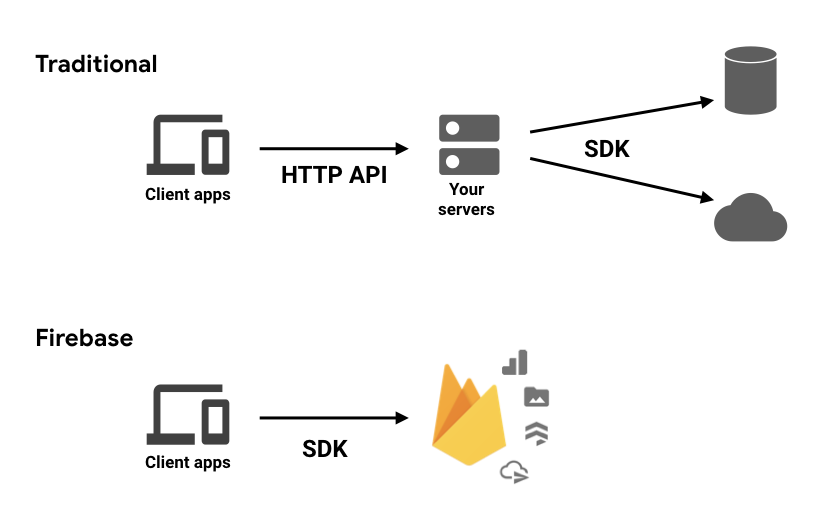
\includegraphics[width=10cm,height=10cm,keepaspectratio]{Images/firebasetradpic.png}
\end{center}

Firebase and other serverless architectures have rapidly emerged as a new technology concept in recent years. Using this Architecture, developers can create a variety of applications for various industries. Many enterprises have already started adopting serverless products, serverless architecture provides computation-light, highly-flexible, stateless applications and more. Developers are constantly on the lookout for more effective ways to maintain the software development lifecycle, doing so introduces new technologies that are accompanied with an increase in productivity. \newline
Serverless architecture was introduced to help businesses focus on application development. With serverless, businesses no longer have to worry about server infrastructure, reducing development costs and shortening the development cycle.\newline

A traditional architecture approach is frequently a large computer or cluster of computers that is accessed over the internet to provide access to information or servers. The machines are commonly located at specific area's around the world depending the size of the company. A traditional approach requires a team to manage these servers that which starts to become a problem what different scales of companies. As you get towards Enterprise sized servers they can become increasingly expensive. Not only do they cost Hundreds of Thousands to millions, you need to have space to house them, a staff of engineers to maintain them. In addition, the average life cycle of a given server is about 5 years. Which means not only do you have to potentially replace your machines, but in the interim you are constrained by the limitations of that machine.\newline
An example of these would be if a websites server does not have the capacity to handle it's increased load, the only traditional solution is to purchase more servers to handle extra volume, or replacing existing servers with a better model. Both have exceptionally high cost and come with large downsides.\newline
\newpage

Serverless Architectures aims to solve these problems. Rather than having one machine to host a job, you can now utilize servers, such as Firebase, Amazon AWS and other cloud hosted databases. All have a huge array of additional features that you opt into to spec out a server that fits your needs and removes the additional costs and headaches of a traditional server.

\begin{figure}[h!]
	\caption{Serverless Evolution}
	\label{image:myImageName}
	\centering
	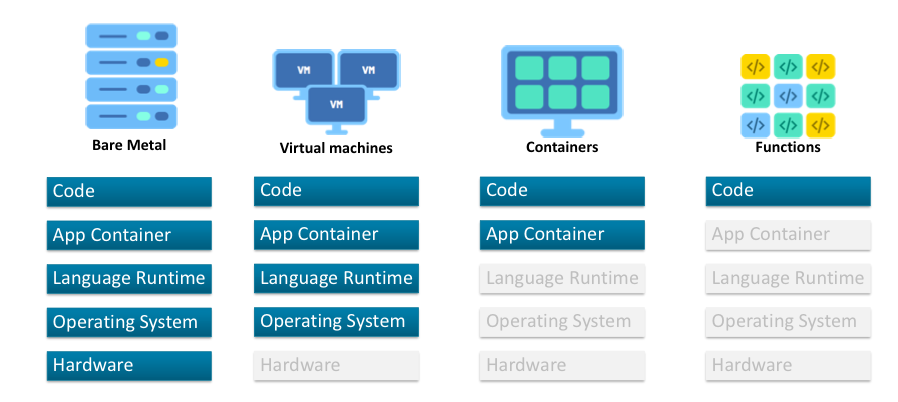
\includegraphics[width=0.8\textwidth]{Images/serverless_evolution.png}
\end{figure}




\subsubsection{Advantages of Serverless}
Advantages Serverless architectures has are the following:
\begin{enumerate}
  \item Providers scale and manages the required resources
  \item Rapid provision of resources in real-time, even for unforeseen peak loads and disproportionate growth
  \item Highly scalable and flexible architecture
  \item Users only need to pay for the resources they use
  \item High error tolerance thanks to flexible hardware infrastructure in the provider’s computer centers
\end{enumerate}

\subsubsection{Disadvantages of Serverless}
Disadvantages Serverless architectures has are the following:
\begin{enumerate}
  \item No access to virtual machines, operating system or runtime environments
  \item Implementing serverless structures is very labor-intensive
  \item Lock-in effect – for example, when changing provider, you generally have to recode all event-based functions
  \item Relatively complex monitoring and debugging process, as in-depth performance, and error analyses are generally not possible
\end{enumerate}
\newpage

As shown Firebase is an excellent option for any developer interested in creating a mobile application, finally i will go over the Pros and Cons of choosing Firebase

\subsubsection{The Pros of Firebase}
\begin{itemize}
    \item \textbf{Databases} - Depending on your budget, Google offers robust databases to use with your apps. Both realtime and Firestore databases can be scaled in terms of size, suggesting a fully secure managed solution, that still provides you easy access to your data via firebase console. Data updates and offline access makes databases usable for real time application, as well as keeping multiple databases in sync
    \item \textbf{Wide selection of products} - Firebase suggest a lot of products to make your application work. You can choose between realtime databases and firestore, store data in the cloud and build serverless applications with the integrated Cloud functions.
    \item \textbf{Free to use for small developers} - Firebase pricing\cite{firebase_pricing} is free as you start with it. This will allow you to understand whether it fits your application and understand all the peculiarities. Once you reach certain amount of database memory or need a specific product, you can choose a different plan around that product or memory you need. You can do this by using the Blaze plan calculator provided on firebase pricing website\cite{firebase_pricing}
    \item \textbf{Excellent Documentation} - The whole firebase platform is extremely well documented. Good technical documentation, API documentation, SDK references, which makes all the products easier to use and accessible for the user. The firebase products page contains all the required information concerning the integration's, available platforms, guidance's, docs, guides and lists supported technologies.
    \item \textbf{Accessible UI and ease of Integration} - Firebase requires minimal programming language knowledge, and suggests integration's via its user interface, it also is integrated into Android Studio which further increases ease of use. While eliminating the need for complex configurations, anyone can set up the application.
    \item \textbf{Google products} - Firebase comes with a Content Delivery Network (CDN) in-built with Google Cloud platform, while also having integration with all google products. A product owned by google also has the advantage of unlikely hood of the company collapsing or not supporting the product frequently.
    
\end{itemize}

\newpage
\subsubsection{The Cons of Firebase}
The cons of firebase are limited and depends on the scope of you project and the size of your company. Some of the cons are currently being fixed through new features that are currently in Beta. For example Firebase Realtime Database, which i used in this project has limitations of not being able to do complex query's and Data Modeling. Google aims to fix this with its new product Firestore. 
\begin{itemize}
    \item \textbf{Firebase Realtime Database limitations} - Realtime Database is used as the main storage for my project, which has cons. One of the mains problems with it, is the limited querying capabilities. Realtime database provides no way to filter capabilities, because the whole Database is a huge JSON file, which makes it pretty difficult to make complex queries.
    \item \textbf{Data Modeling} - Firebase Realtime Database and it data modeling as a problem where because of "Database as a single JSON file" structure,m you can't implement relations between data items.
    \item \textbf{Locked into a vendor} - This is a wide problem with BaaS solutions in general, not having the ability to migrate data to another platform can be considered a con.
     \item \textbf{Support for iOS} - While firebase is a cross-platform product, it concentrates more on Android mobile platform being that its a google product. Android Studio easily integrates all Firebase products such as Test Lab, Auth etc. While iOS devices are lacking behind on such integration's.
\end{itemize}
\newpage

%----------------------------------------------------------------------------------------
% PICASSO IMAGE HANDLING
%----------------------------------------------------------------------------------------
\subsection{Picasso}
\par
\medskip
\begin{center}
    
\includegraphics[width=10cm,height=10cm,keepaspectratio]{Images/picasso.png}
\end{center}
Picasso is a powerful image downloading and caching library, it is widely used and requires very little code to implement.
This is used because working with images in android is difficult, you need to work with network requests, caching, background threads and decoding \& encoding of image which uses a lot of memory. Picasso hides all this and adds additional features like resizing images while being memory efficient.\newline

Images add much-needed context and visual flair to Android applications. Picasso allows for hassle-free image loading in your application—often in one line of code!

\begin{lstlisting}
Picasso.get().load("http://i.imgur.com/DvpvklR.png").into(imageView);
\end{lstlisting}


Many common pitfalls of image loading on Android are handled automatically by Picasso:
\begin{itemize}
    \item Handling ImageView recycling and download cancellation in an adapter.
    \item Complex image transformations with minimal memory use.
    \item Automatic memory and disk caching.
\end{itemize}

\begin{center}
    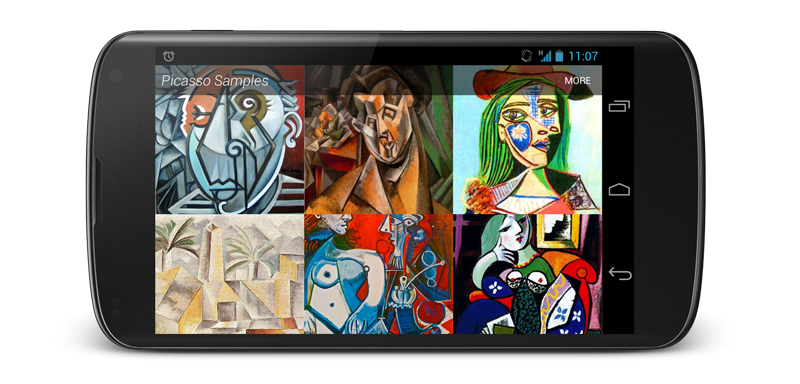
\includegraphics[width=10cm,height=10cm,keepaspectratio]{Images/picassoex1.png}
\end{center}
\newpage

\subsubsection{Features}

\textbf{ADAPTER DOWNLOADS}\newline
Adapter re-use is automatically detected and the previous download canceled.
\begin{lstlisting}
@Override public void getView(int position, View convertView, ViewGroup parent) {
  SquaredImageView view = (SquaredImageView) convertView;
  if (view == null) {
    view = new SquaredImageView(context);
  }
  String url = getItem(position);

  Picasso.get().load(url).into(view);
}
\end{lstlisting}


\textbf{IMAGE TRANSFORMATIONS}\newline

Transform images to better fit into layouts and to reduce memory size.
\begin{lstlisting}
Picasso.get()
  .load(url)
  .resize(50, 50)
  .centerCrop()
  .into(imageView)
\end{lstlisting}
\textbf{Can also specify custom transformations for more advanced effects.}
\begin{lstlisting}
public class CropSquareTransformation implements Transformation {
  @Override public Bitmap transform(Bitmap source) {
    int size = Math.min(source.getWidth(), source.getHeight());
    int x = (source.getWidth() - size) / 2;
    int y = (source.getHeight() - size) / 2;
    Bitmap result = Bitmap.createBitmap(source, x, y, size, size);
    if (result != source) {
      source.recycle();
    }
    return result;
  }

  @Override public String key() { return "square()"; }
}
\end{lstlisting}
Pass an instance of this class to the transform method.
\newpage

\textbf{PLACE HOLDERS}\newline

Picasso supports both download and error placeholders as optional features.
\begin{lstlisting}
Picasso.get()
    .load(url)
    .placeholder(R.drawable.user_placeholder)
    .error(R.drawable.user_placeholder_error)
    .into(imageView);
\end{lstlisting}
A request will be retried three times before the error placeholder is shown.\newline

\textbf{RESOURCE LOADING}\newline

Resources, assets, files, content providers are all supported as image sources.
\begin{lstlisting}
Picasso.get().load(R.drawable.landing_screen).into(imageView1);
Picasso.get().load("file:///android_asset/DvpvklR.png").into(imageView2);
Picasso.get().load(new File(...)).into(imageView3);
\end{lstlisting}

\textbf{DEBUG INDICATORS}\newline

For development you can enable the display of a colored ribbon which indicates the image source. Call setIndicatorsEnabled(true) on the Picasso instance.
\begin{center}
    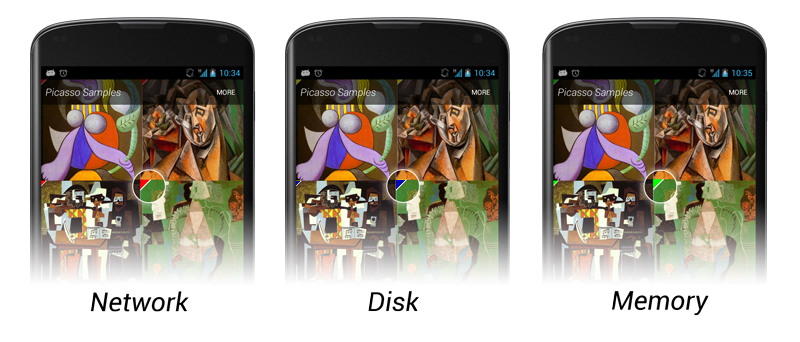
\includegraphics[width=12cm,height=12 cm,keepaspectratio]{Images/picassodebug.png}
\end{center}
\newpage

%----------------------------------------------------------------------------------------
% NATIVE APPLICATIONS
%----------------------------------------------------------------------------------------
\subsection{Native Applications}
\par
\medskip
\begin{center}
    
\includegraphics[width=12cm,height=12cm,keepaspectratio]{Images/nativeapp2.png}
\end{center}

blah..


\subsubsection{Advantages}
\begin{itemize}
    \item \textbf{Shift from Java to Kotlin} - Kotlin
    \item \textbf{Hard to find experienced developers} - asdas
    \item \textbf{Limited learning resources} - Although
\end{itemize}
\subsubsection{Disadvantages}
\begin{itemize}
    \item \textbf{Shift from Java to Kotlin} - Kotlin
    \item \textbf{Hard to find experienced developers} - asdas
    \item \textbf{Limited learning resources} - Although
\end{itemize}

\subsection{Hybrid Applications}
\par
\medskip
\begin{center}
    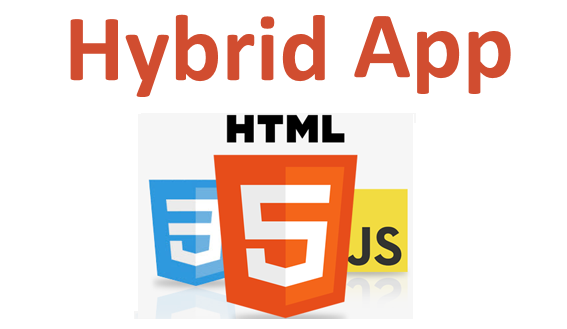
\includegraphics[width=12cm,height=12cm,keepaspectratio]{Images/hybridapp.png}
\end{center}

blah..


\subsubsection{Advantages}
\begin{itemize}
    \item \textbf{Shift from Java to Kotlin} - Kotlin
    \item \textbf{Hard to find experienced developers} - asdas
    \item \textbf{Limited learning resources} - Although
\end{itemize}
\subsubsection{Disadvantages}
\begin{itemize}
    \item \textbf{Shift from Java to Kotlin} - Kotlin
    \item \textbf{Hard to find experienced developers} - asdas
    \item \textbf{Limited learning resources} - Although
\end{itemize}

\subsection{Hybrid vs Native Applications}
\par
\medskip
\begin{center}
    
\includegraphics[width=12cm,height=12cm,keepaspectratio]{Images/hybridvnative.png}
\end{center}

blah..


\subsubsection{Advantages}
\begin{itemize}
    \item \textbf{Shift from Java to Kotlin} - Kotlin
    \item \textbf{Hard to find experienced developers} - asdas
    \item \textbf{Limited learning resources} - Although
\end{itemize}
\subsubsection{Disadvantages}
\begin{itemize}
    \item \textbf{Shift from Java to Kotlin} - Kotlin
    \item \textbf{Hard to find experienced developers} - asdas
    \item \textbf{Limited learning resources} - Although
\end{itemize}

\begin{figure}[h!]
	\caption{Hybrid Application}
	\label{image:myImageName}
	\centering
	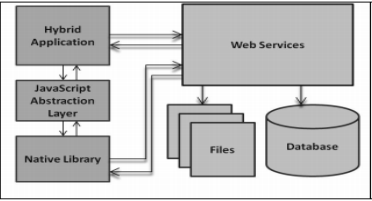
\includegraphics[width=1\textwidth]{Images/hybrid_dev_img.PNG}
\end{figure}

\chapter{System Design}

\section{Chapter Introduction}
In this section I will discuss the architecture of the application. I will discuss the components of an android application mainly Android Activities and the tops that come with Activities; Fragments, Activity lifecycle, persistence, process lifecycle etc. I will also discuss how the Front-End communicates with the Back-End after explaining of activities work.

\section{Introduction to System}
This application was made using Kotlin with Android Studio. My application uses Single Activity App Architecture, which is recommended by Google as the best way to make a Native Android Application\cite{android_single_activity_blog}

\section{Android Activities}
An activity is a single, focused thing that the user can do. Almost all activities interact with the user, so the Activity class takes care of creating a window for you in which you can place your UI with setContentView. While activities are often presented to the user as full-screen windows, they can also be used in other ways: as floating windows (via a theme with android.R.attr\#windowIsFloating set), Multi-Window mode or embedded into other windows.\cite{android_activity_docs} There are two methods almost all subclasses of Activity will implement: 

\begin{itemize}
    \item onCreate  is where you initialize your activity. Most importantly, here you will usually call setContentView(int) with a layout resource defining your UI, and using findViewById to retrieve the widgets in that UI that you need to interact with programmatically.
    \item onPause is where you deal with the user pausing active interaction with the activity. Any changes made by the user should at this point be committed (usually to the android.content.ContentProvider holding the data). In this state the activity is still visible on screen.
\end{itemize}

To be of use with Context.startActivity(), all activity classes must have a corresponding <activity> declaration in their package's \textbf{AndroidManifest.xml.}

\subsection{Fragments}
A Fragment represents a behavior or a portion of user interface in a FragmentActivity. You can combine multiple fragments in a single activity to build a multi-pane UI and reuse a fragment in multiple activities. You can think of a fragment as a modular section of an activity, which has its own lifecycle, receives its own input events, and which you can add or remove while the activity is running (sort of like a "sub activity" that you can reuse in different activities).\cite{android_activity_fragments}\newline

A fragment must always be hosted in an activity and the fragment's lifecycle is directly affected by the host activity's lifecycle. For example, when the activity is paused, so are all fragments in it, and when the activity is destroyed, so are all fragments. However, while an activity is running, you can manipulate each fragment independently, such as add or remove them. When you perform such a fragment transaction, you can also add it to a back stack that's managed by the activity—each back stack entry in the activity is a record of the fragment transaction that occurred. The back stack allows the user to reverse a fragment transaction (navigate backwards), by pressing the Back button.\cite{android_activity_fragments}\newline

When you add a fragment as a part of your activity layout, it lives in a ViewGroup inside the activity's view hierarchy and the fragment defines its own view layout. You can insert a fragment into your activity layout by declaring the fragment in the activity's layout file, as a <fragment> element, or from your application code by adding it to an existing ViewGroup.\cite{android_activity_fragments}\newline

\newpage
\begin{figure}[h!]
	\caption{Android app which uses Architecture components \cite{android_guide_arc}}
	\label{image:myImageName}
	\centering
	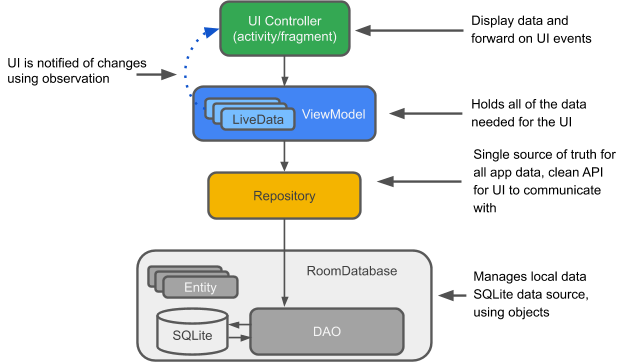
\includegraphics[width=1\textwidth]{Images/android_app_arc.png}
\end{figure}	

\subsection{Creating a Fragment}

Example of Fragment in Project to create the Navigation Bars:\newline

\textbf{HomeViewModel}
\begin{minted}{kotlin}
class HomeViewModel : ViewModel() {

    private val _text = MutableLiveData<String>().apply {
        value = "This is home Fragment"
    }
    val text: LiveData<String> = _text
}
\end{minted}


\textbf{HomeFragment}
\begin{minted}{kotlin}
class HomeFragment : Fragment() {

    private lateinit var homeViewModel: HomeViewModel

    override fun onCreateView(
        inflater: LayoutInflater,
        container: ViewGroup?,
        savedInstanceState: Bundle?
    ): View? {
        homeViewModel =
            ViewModelProviders.of(this).get(HomeViewModel::class.java)
        val root = inflater.inflate(R.layout.fragment_home, container, false)
        val textView: TextView = root.findViewById(R.id.text_home)
        homeViewModel.text.observe(this, Observer {
            textView.text = it
        })
        return root
    }
}
\end{minted}

After creating a fragment you then need to declare it inside an activity layout file
\begin{minted}{kotlin}
<?xml version="1.0" encoding="utf-8"?>
<androidx.constraintlayout.widget.ConstraintLayout xmlns:android="http://schemas.android.com/apk/res/android"
    xmlns:app="http://schemas.android.com/apk/res-auto"
    android:layout_width="match_parent"
    android:layout_height="match_parent">

    <TextView
        android:id="@+id/text_home"
        android:layout_width="match_parent"
        android:layout_height="wrap_content"
        android:layout_marginStart="8dp"
        android:layout_marginTop="8dp"
        android:layout_marginEnd="8dp"
        android:textAlignment="center"
        android:textSize="20sp"
        app:layout_constraintEnd_toEndOf="parent"
        app:layout_constraintStart_toStartOf="parent"
        app:layout_constraintTop_toTopOf="parent" />
</androidx.constraintlayout.widget.ConstraintLayout>
\end{minted}

\subsection{Communicating with a Activity}

Although a \textbf{Fragment} is implemented as an object that's independent from a \textbf{FragmentActivity} and can be used inside multiple activities, a given instance of a fragment is directly tied to the activity that hosts it.

Specifically, the fragment can access the FragmentActivity instance with getActivity() and easily perform tasks such as find a view in the activity layout:

\begin{minted}{kotlin}
val listView: View? = activity?.findViewById(R.id.list)
\end{minted}

Likewise, your activity can call methods in the fragment by acquiring a reference to the Fragment from FragmentManager, using findFragmentById() or findFragmentByTag(). For example:
\begin{minted}{kotlin}
val fragment = supportFragmentManager.findFragmentById(R.id.example_fragment) as ExampleFragment
\end{minted}

\section{Implementation of Activities}
Here i will  describe a list of Activities and their functionality with code examples.

\subsection{List of Activities}
Each of the following subsections describe the anatomy of each Activity and will discuss their purpose and the code used to implement each component.
\subsection{Main Activity}
The MainActivity contains all the code that will appear when first launching the application. It contains Login and Register button as well as the OnClickListener for those buttons. The MainActivity also contains the code for the navigation controller between fragments.
\begin{minted}{kotlin}
val drawerLayout: DrawerLayout = findViewById(R.id.drawer_layout)
val navView: NavigationView = findViewById(R.id.nav_view)
val navController = findNavController(R.id.nav_host_fragment)

// Passing each menu ID as a set of Ids because each
    // menu should be considered as top level destinations.
    appBarConfiguration = AppBarConfiguration(
        setOf(
            R.id.nav_home, R.id.nav_gallery, R.id.nav_slideshow,
            R.id.nav_tools, R.id.nav_share, R.id.nav_send
        ), drawerLayout
    )
    setupActionBarWithNavController(navController, appBarConfiguration)
    navView.setupWithNavController(navController)
} //onCreate end

override fun onCreateOptionsMenu(menu: Menu): Boolean {
    // Inflate the menu; this adds items to the action bar if it is present.
    menuInflater.inflate(R.menu.main, menu)
    return true
}

override fun onSupportNavigateUp(): Boolean {
    val navController = findNavController(R.id.nav_host_fragment)
    return navController.navigateUp(appBarConfiguration) || super.onSupportNavigateUp()
}

\end{minted}

%----------------------------------------------------------------------------------------
% REGISTER
%----------------------------------------------------------------------------------------
\newpage
\subsection{Register}
The Register Activity is the activity that is triggered when the user clicks on Join Now Button, the RegisterAcivity is used to create an account on the Firebase Database and to also verify that the Phone Number given is unique to the database.\newline

Similar to the LoginAcivity there are four steps that i will explain in four different subsubsections. 


\subsubsection{The Trigger Event}
1. The user clicks on the Join Now Button, this will activate a OnClickListener in the MainAcivity
\begin{minted}{kotlin}
// This code is triggered by a OnClickListener, 
// once triggered the view context of the app will move from MainAcivity to RegisterActivity
// RegisterActivity::class.java
joinNowButton.setOnClickListener{view ->
    val intent = Intent(view.context, RegisterActivity::class.java)
    view.context.startActivity(intent)
}
\end{minted}

\subsubsection{onCreate and Variables}
2. Once the user triggers the event the UI will be shown
\begin{minted}{kotlin}
class RegisterActivity : AppCompatActivity() {

    private lateinit var CreateAccountButton: Button
    private lateinit var InputName: EditText
    private lateinit var InputPhoneNumber: EditText
    private lateinit var InputPassword: EditText
    private lateinit var loadingBar: ProgressDialog

    override fun onCreate(savedInstanceState: Bundle?) {
        super.onCreate(savedInstanceState)
        setContentView(R.layout.activity_register)

        CreateAccountButton = findViewById(R.id.register_btn)
        InputName = findViewById(R.id.register_user_name_input)
        InputPhoneNumber = findViewById(R.id.register_phone_number_input)
        InputPassword = findViewById(R.id.register_password_input)
        loadingBar = ProgressDialog(this)

        CreateAccountButton.setOnClickListener{
            CreateAccount()
        } }
\end{minted}

\subsubsection{Creating a Account}
3. Once the user clicks the Join Now Button another OnClickListener will trigger which calls this method to Create an Account, CreateAccount() will also call validatePhoneNumber to valid the user's phone number input. This is used to remove any duplicate phone number as its the Primary Key in the Database. 
\begin{minted}{kotlin}
  private fun CreateAccount() {
    var name = InputName.text.toString()
    var phone = InputPhoneNumber.text.toString()
    var password = InputPassword.text.toString()

    if (TextUtils.isEmpty(name)){
        Toast.makeText(this, "Write your name... ", Toast.LENGTH_SHORT).show()
    }
    else if (TextUtils.isEmpty(phone)){
        Toast.makeText(this, "Write your phone number... ", Toast.LENGTH_SHORT).show()
    }
    else if (TextUtils.isEmpty(password)){
        Toast.makeText(this, "Write your password... ", Toast.LENGTH_SHORT).show()
    }
    else{
        loadingBar.setTitle("Create Account")
        loadingBar.setMessage("Please wait, while we validate your information.")
        loadingBar.setCanceledOnTouchOutside(false)
        loadingBar.show()

        validatePhoneNumber(name, phone, password)

    }
}
\end{minted}

\subsubsection{Account Verification}
4. This is the last step for the user to register a account. This method will enter the users input into the Firebase Database and will also check if any users contain the same Phone Number. If a user has the same phone number the account will not be created and the user will be prompted to enter a new number.
The reason for this is the Phone Number is the Primary Key in the Database and the Phone Number is also setup for phone authentication with google products, so having multiple accounts with the same number would serve no purpose so eliminating this is the best option.\newline \newline \newline

\begin{minted}{kotlin}
//WORKS AFTER TESTING - SCHEMA USERS - KEY PHONENUMBER - DETAILS NAME:< PASSWORD:< PHONE:
private fun validatePhoneNumber(name: String, phone: String, password: String) {

val RootRef:DatabaseReference
RootRef = FirebaseDatabase.getInstance().getReference()

RootRef.addListenerForSingleValueEvent(object: ValueEventListener{
override fun onDataChange(dataSnapshot: DataSnapshot) {
    //val post = dataSnapshot.getValue(String::class.java)
    //Update the UI with received data
    if (!(dataSnapshot.child("Users").child(phone).exists())){
        val childUpdates = HashMap<String, Any>()
        childUpdates.put("phone", phone)
        childUpdates.put("password", password)
        childUpdates.put("name", name)

        RootRef.child("Users").child(phone).updateChildren(childUpdates)
            .addOnCompleteListener(object: OnCompleteListener<Void>{
                override fun onComplete(@NonNull task: Task<Void>){
                    if (task.isSuccessful()){
                        Toast.makeText(this@RegisterActivity,
                        "Your Account has been created.", Toast.LENGTH_SHORT).show()
                        loadingBar.dismiss()

                        val intent = Intent(this@RegisterActivity,
                        LoginActivity::class.java)
                        startActivity(intent)
                    }//if
                    else{
                        loadingBar.dismiss()
                        Toast.makeText(this@RegisterActivity,
                        "Network Error: Please Try Again...", Toast.LENGTH_SHORT).show()
                    }
                }//onComplete
            })//addOnCompleteListener
    }//Data
    else{
        Toast.makeText(this@RegisterActivity,
        "This " + phone + "already exists.", Toast.LENGTH_SHORT).show()
        loadingBar.dismiss()
        Toast.makeText(this@RegisterActivity,
        "Please try another number", Toast.LENGTH_SHORT).show()

        val intent = Intent(this@RegisterActivity, LoginActivity::class.java)
        startActivity(intent)
    } }//onDataChange
\end{minted}
%----------------------------------------------------------------------------------------
% LOGIN
%----------------------------------------------------------------------------------------
\subsection{Login}
The login Activity is the activity that the user will see when clicking the Login button at the home page. The activity features a welcome message and prompts user to either Login or create a new account. From here depending on which button is pressed two things can happen either a Login Button is click or a Join Now button is clicked here i will explain of the LoginAcivity works.\newline

There are four steps to this that i will explain in four different subsubsections.

%\newpage
\subsubsection{The Trigger Event}
1. The user clicks on the Login Button, this will activate a OnClickListener in the MainAcivity.
\begin{minted}{kotlin}
// This code is triggered by a OnClickListener, 
// once triggered the view context of the app will move from MainAcivity to LoginAcivity
// LoginActivity::class.java
loginButton.setOnClickListener{view ->
    val intent = Intent(view.context, LoginActivity::class.java)
    view.context.startActivity(intent)
}
\end{minted}

\subsubsection{onCreate and Variables}
2. Once the user triggers the event the UI will be shown

\begin{minted}{kotlin}
class LoginActivity : AppCompatActivity() {

    private lateinit var InputPassword: EditText
    private lateinit var InputPhoneNumber: EditText
    private lateinit var LoginButton: Button
    private lateinit var loadingBar: ProgressDialog
    private val parentDbName = "Users"

    override fun onCreate(savedInstanceState: Bundle?) {
        super.onCreate(savedInstanceState)
        setContentView(R.layout.activity_login)

        LoginButton = findViewById(R.id.login_btn)
        InputPhoneNumber = findViewById(R.id.login_phone_number_input)
        InputPassword = findViewById(R.id.login_password_input)
        loadingBar = ProgressDialog(this)
        
        LoginButton.setOnClickListener{
            LoginUser()
        }
    }//onCreate
\end{minted}
\newpage
\subsubsection{Login the User}
3. Once user now clicks the Login Button another OnClickListener will trigger which calls this method to login, LoginUser will also call AllowAccessToAccount to verify the user in the Firebase DB.
\begin{minted}{kotlin}
private fun LoginUser() {
    var phone = InputPhoneNumber.text.toString()
    var password = InputPassword.text.toString()

    if (TextUtils.isEmpty(phone)){
        Toast.makeText(this, "Write your phone number... ", Toast.LENGTH_SHORT).show()
    }
    else if (TextUtils.isEmpty(password)){
        Toast.makeText(this, "Write your password... ", Toast.LENGTH_SHORT).show()
    }
    else{
        loadingBar.setTitle("Login Account")
        loadingBar.setMessage("Please wait, while we validate your information.")
        loadingBar.setCanceledOnTouchOutside(false)
        loadingBar.show()
        
        AllowAccessToAccount(phone, password)
    }
}//LoginUser
\end{minted}
\begin{figure}[h!]
	\caption{Login View - Activity\_login\.XML}
	\label{image:myImageName}
	\centering
	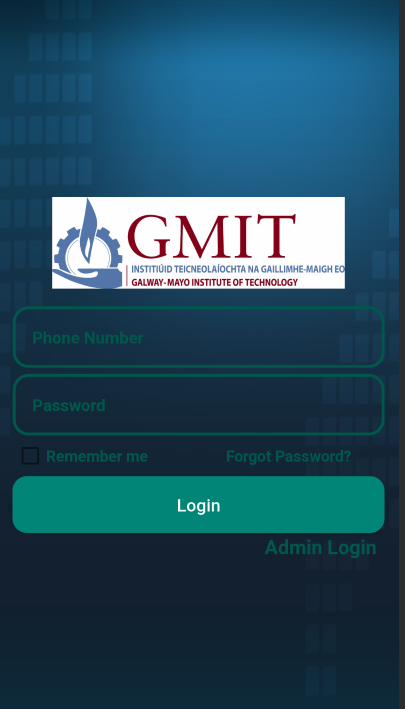
\includegraphics[width=0.35\textwidth]{Images/login_view.png}
	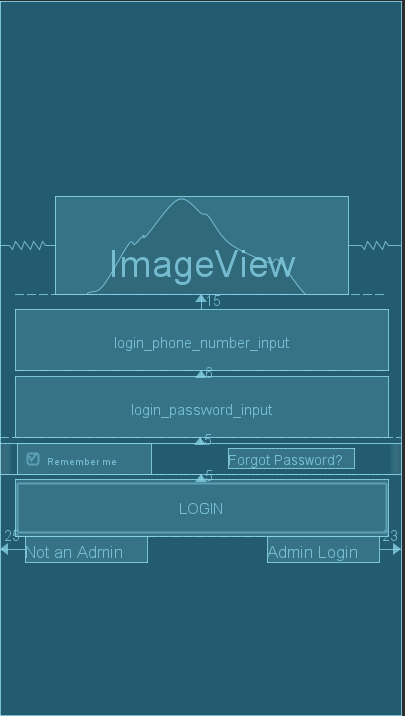
\includegraphics[width=0.35\textwidth]{Images/login_deisign.png}
\end{figure}
\newpage
\subsubsection{Login Verification and Remember me}
4. This is the last step for the user to Login. this method will called in the LoginUser method to verify that the details the user inputs are valid. If they're valid the user will be sent to the HomeAcivity page where they will see Products.
\begin{minted}{kotlin}
private fun allowAccessToAccount(phone: String, password: String) {

if (checkBoxRememberMe.isChecked){
    Paper.book().write(Prevalent.UserPhoneKey, phone)
    Paper.book().write(Prevalent.UserPasswordKey, password)
}
val RootRef: DatabaseReference
RootRef = FirebaseDatabase.getInstance().getReference()
RootRef.addListenerForSingleValueEvent(object: ValueEventListener {

    override fun onDataChange(dataSnapshot: DataSnapshot) {
        //var userData:Users
        if(dataSnapshot.child(parentDbName).child(phone).exists()){
            var usersData = dataSnapshot.child(parentDbName).child(phone).getValue(Users::class.java)

            if (usersData?.getPhone().equals(phone)){
                if (usersData?.getPassword().equals(password)){
                    if(parentDbName.equals("Admins")){
                        Toast.makeText(this@LoginActivity, "Admin Login Successful", Toast.LENGTH_SHORT).show()
                        loadingBar.dismiss()
                        //Sends user to AdminActivity
                        val intent = Intent(this@LoginActivity, AdminPanelActivity::class.java)
                        startActivity(intent)
                    }
                    else if(parentDbName.equals("Users")){
                        Toast.makeText(this@LoginActivity, "Login Successful", Toast.LENGTH_SHORT).show()
                        loadingBar.dismiss()
                        //Sends user to HomeActivity
                        val intent = Intent(this@LoginActivity, HomeActivity::class.java)
                        Prevalent.currentOnlineUser = usersData!!
                        startActivity(intent)
                    }
                }
                else{
                    Toast.makeText(this@LoginActivity, "Password is Incorrect...", Toast.LENGTH_SHORT).show()
                    loadingBar.dismiss()
                }
            }//getPhone if
        }
        else{
            Toast.makeText(this@LoginActivity, "Account with this " + phone + " Number does not exist", Toast.LENGTH_SHORT).show()
       
\end{minted}
\newpage
\subsection{Navigation}

The Navigation for my project is created using the Navigation Drawer Activity in combination with Fragments

\subsubsection{Setting up Drawer Resources}
First you must create an drawer resource. Here i will show aciviity\_home\_drawer\.xml

\begin{minted}{kotlin}
<menu xmlns:android="http://schemas.android.com/apk/res/android"
    xmlns:tools="http://schemas.android.com/tools"
    tools:showIn="navigation_view">

    <group android:checkableBehavior="single">
        <item
            android:id="@+id/nav_home"
            android:icon="@drawable/ic_menu_camera"
            android:title="Home" />
        <item
            android:id="@+id/nav_gallery"
            android:icon="@drawable/ic_menu_gallery"
            android:title="Cart" />
        <item
            android:id="@+id/nav_slideshow"
            android:icon="@drawable/ic_menu_slideshow"
            android:title="Orders" />
        <item
            android:id="@+id/nav_tools"
            android:icon="@drawable/ic_menu_manage"
            android:title="Categories" />
    </group>

    <item android:title="Settings">
        <menu>
            <item
                android:id="@+id/nav_share"
                android:icon="@drawable/ic_menu_share"
                android:title="Settings" />
            <item
                android:id="@+id/nav_send"
                android:icon="@drawable/ic_menu_send"
                android:title="Logout" />
        </menu>
    </item>

</menu>

\end{minted}

\subsubsection{Define Fragments}
After this next is to define fragments that will be displayed within the Navigation Activity;.
These fragments are created in the ui folder each with a View\-Model and a host Fragment.
Once created we then need to create Mobile\_navigation\.xml which is used to navigation between each fragment.
\begin{minted}{kotlin}
    <fragment
        android:id="@+id/nav_home"
        android:name="com.example.ecommerce.ui.home.HomeFragment"
        android:label="@string/menu_home"
        tools:layout="@layout/fragment_home" />

    <fragment
        android:id="@+id/nav_gallery"
        android:name="com.example.ecommerce.ui.cart.CartFragment"
        android:label="@string/menu_gallery"
        tools:layout="@layout/fragment_cart" />

    <fragment
        android:id="@+id/nav_slideshow"
        android:name="com.example.ecommerce.ui.orders.OrdersFragment"
        android:label="@string/menu_slideshow"
        tools:layout="@layout/fragment_orders" />

    <fragment
        android:id="@+id/nav_tools"
        android:name="com.example.ecommerce.ui.categories.CategoriesFragment"
        android:label="@string/menu_tools"
        tools:layout="@layout/fragment_tools" />

    <fragment
        android:id="@+id/nav_share"
        android:name="com.example.ecommerce.ui.settings.SettingsFragment"
        android:label="@string/menu_share"
        tools:layout="@layout/fragment_settings" >
    </fragment>

    <fragment
        android:id="@+id/nav_send"
        android:name="com.example.ecommerce.ui.logout.LogoutFragment"
        android:label="@string/menu_send"
        tools:layout="@layout/fragment_logout" />
</navigation>
\end{minted}

\subsubsection{Navigation Host Fragment}
Once we've create all the Fragments and connected them with the Navigation View we must choose a Nav Host Fragment. This is basically the highest level activity of the navigation view, anything created on this Activity will appear on other views when you change to other Fragments in the navigation. 

\begin{minted}{kotlin}
    <fragment
        android:id="@+id/nav_host_fragment"
        android:name="androidx.navigation.fragment.NavHostFragment"
        android:layout_width="match_parent"
        android:layout_height="match_parent"
        app:defaultNavHost="true"
        app:navGraph="@navigation/mobile_navigation" />
\end{minted}


\begin{figure}[h!]
	\caption{Navigation View - Activity\_home\.XML}
	\label{image:myImageName}
	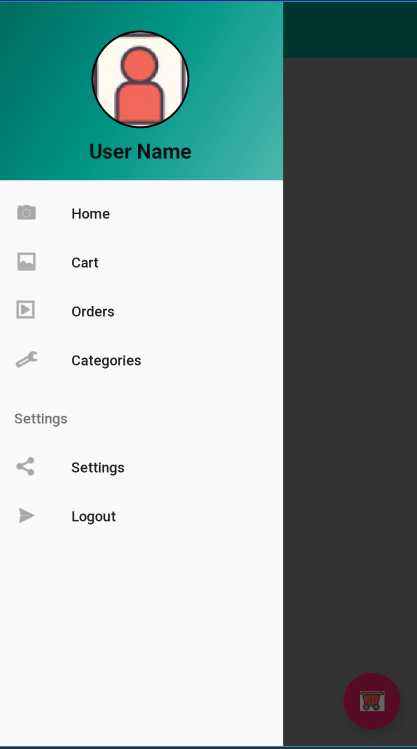
\includegraphics[width=0.5\textwidth]{Images/nav_activity_homexml.png}
	
\includegraphics[width=0.5\textwidth]{Images/nav_activity_home_view_xml.png}
\end{figure}

\subsubsection{Setup Navigation in Activity}
Setting up the Navigation within the Activity does not take up much code in kotlin compared to Java.\newline

\textbf{First i initialize all the needed Views and setup the navController}

\begin{minted}{kotlin}
val toolbar: Toolbar = findViewById(R.id.toolbar)
setSupportActionBar(toolbar)
val drawerLayout: DrawerLayout = findViewById(R.id.drawer_layout)
val navView: NavigationView = findViewById(R.id.nav_view)
val navController = findNavController(R.id.nav_host_fragment)
setupActionBarWithNavController(navController, appBarConfiguration)
navView.setupWithNavController(navController)
\end{minted}

I will also attach a addOnDestinationChangedListener to the navController.

\begin{minted}{kotlin}
navController.addOnDestinationChangedListener { _, destination, _ ->
            when {
                destination.id == R.id.nav_share -> {
                    toolbar.visibility = View.VISIBLE
                    recyclerView.visibility = View.GONE
                }
                destination.id == R.id.nav_tools -> {
                    toolbar.visibility = View.VISIBLE
                    recyclerView.visibility = View.GONE
                }
                destination.id == R.id.nav_slideshow -> {
                    toolbar.visibility = View.VISIBLE
                    recyclerView.visibility = View.GONE
                }
                destination.id == R.id.nav_gallery -> {
                    toolbar.visibility = View.VISIBLE
                    recyclerView.visibility = View.GONE
                }
                destination.id == R.id.nav_send -> {
                    toolbar.visibility = View.VISIBLE
                    recyclerView.visibility = View.GONE
                    
                    Paper.book().destroy()
                    val intent = Intent(this, LoginActivity::class.java)
                    intent.flags = Intent.FLAG_ACTIVITY_NEW_TASK or Intent.FLAG_ACTIVITY_CLEAR_TASK
                    startActivity(intent)
                }
                else -> {
                    toolbar.visibility = View.VISIBLE
                    recyclerView.visibility = View.VISIBLE
                }
\end{minted}
After implementing all of these code snippets the Navigation Drawer is now fully connected and ready to have code implemented. The Navigation will display as shown in Figure \ref{image:myImageName}

\subsection{Admin}

The admin portion of my project is entered through the LoginActivity where the user must choose the admin login to reach the AdminPanelActivity.\newline

The Admin feature consists of two different Activities, AdminActivity \& AdminPanelActivity

\subsubsection{AdminPanelActivity}
The AdminPanelActivity is the first View the user will see after logging in with an Admin Account. This Panel is used for the user to add products to the application store. The panel consists of Twelve different categories, each being a different category for the store (Men's clothes, Women's Clothes, furniture, phones etc.)

\begin{figure}[h!]
	\caption{Admin Panel View - Activity\_admin\_panel\.XML}
	\label{image:myImageName}
	\centering
	
\includegraphics[width=0.45\textwidth]{Images/admin_panel_view.png}
	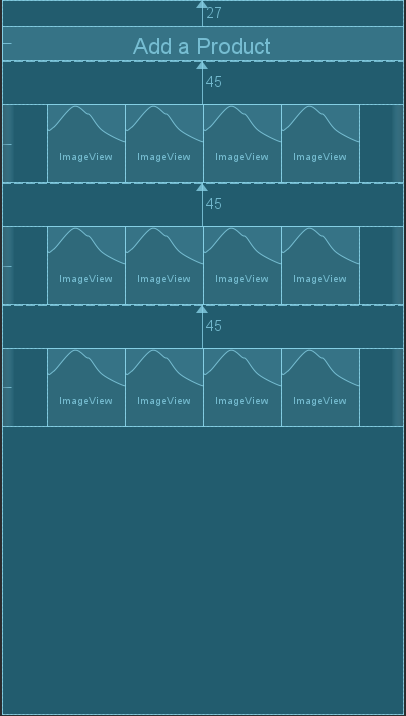
\includegraphics[width=0.45\textwidth]{Images/admin_panel_design.png}
\end{figure}

Each ImageView shown in Figure \ref{image:myImageName} as its on setOnClickListener which will pass on the Category and the value of the Categoryt to the AdminActivity when an imageview is chosen.

\begin{minted}{kotlin}
        //*******************************************************************
        //Layout 3 OnClickListeners - tablets, phones, books, gaming
        //*******************************************************************

        tablets.setOnClickListener{
            val intent = Intent(this, AdminActivity::class.java)
            intent.putExtra("category", "Tablets")
            startActivity(intent)
        }
        phones.setOnClickListener{
            val intent = Intent(this, AdminActivity::class.java)
            intent.putExtra("category", "Phones")
            startActivity(intent)
        }
        books.setOnClickListener{
            val intent = Intent(this, AdminActivity::class.java)
            intent.putExtra("category", "Books")
            startActivity(intent)
        }
        gaming.setOnClickListener{
            val intent = Intent(this, AdminActivity::class.java)
            intent.putExtra("category", "Gaming")
            startActivity(intent)
        }
\end{minted}

\newpage
\subsubsection{AdminActivity}
After Choosing a Category in the AdminPanelActivity the setOnClickListener will send the user to the AdminActivity here the Products are added with a Name, Desc and Price. The user will also choose the image that will be displayed in the RecyclerView after a user logs in.

\begin{figure}[h!]
	\caption{Admin Panel View - Activity\_admin\_panel\.XML}
	\label{image:myImageName}
	\centering
	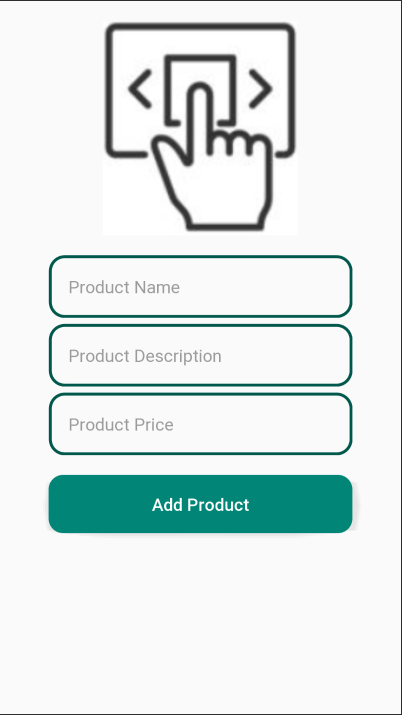
\includegraphics[width=0.45\textwidth]{Images/admin_view.png}
	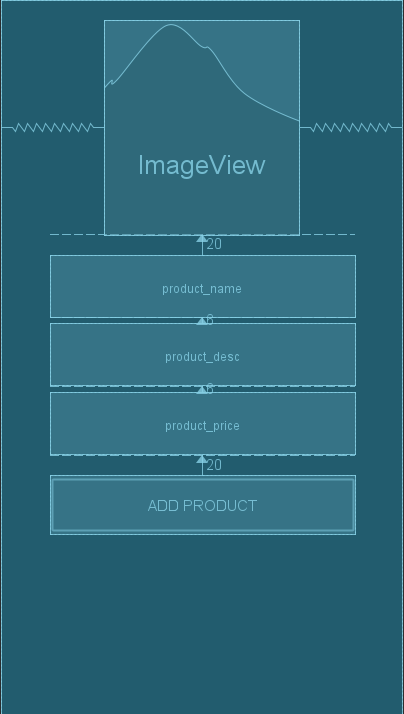
\includegraphics[width=0.45\textwidth]{Images/admin_design.png}
\end{figure}


\subsubsection{Saving Products to Database}

1. Initialize all the needed Views
\begin{minted}{kotlin}
    CategoryName = getIntent().getExtras()?.get("category").toString()
    ProductImageRef = FirebaseStorage.getInstance().reference.child("Product Images")
    ProductRef = FirebaseDatabase.getInstance().reference.child("Products")
    InputProductImage = findViewById(R.id.select_product)
    InputProductName = findViewById(R.id.product_name)
    InputProductDesc =  findViewById(R.id.product_desc)
    InputProductPrice = findViewById(R.id.product_price)
    AddProductButton =  findViewById(R.id.add_new_product)
    loadingBar = ProgressDialog(this)
\end{minted}

2. Set up OnClickListerners
\begin{minted}{kotlin}
    //OnClickListeners
    InputProductImage.setOnClickListener{
        openProducts()
    }

    AddProductButton.setOnClickListener{
        validateProducts()
    }
\end{minted}

3. Validation
Before saving any to the database, validation to be sure all fields are appropriately filled is needed. If all fields are not empty the storeProductInfo() function will be called to store the details
\begin{minted}{kotlin}
    private fun validateProducts() {
    Desc = InputProductDesc.getText().toString()
    Price = InputProductPrice.getText().toString()
    Prod_Name = InputProductName.getText().toString()

    if(TextUtils.isEmpty(Desc)){
        Toast.makeText(this, "Please write a Product Desc ", Toast.LENGTH_SHORT).show()
    }
    else if(TextUtils.isEmpty(Price)){
        Toast.makeText(this, "Please write a Product Price ", Toast.LENGTH_SHORT).show()
    }
    else if(TextUtils.isEmpty(Prod_Name)){
        Toast.makeText(this, "Please write a Product Name ", Toast.LENGTH_SHORT).show()
    }
    else{
        storeProductInfo()
    }
}
\end{minted}

4. Storing the Product Details

First we must declare all the necessary variables

\begin{minted}{kotlin}
private fun storeProductInfo() {
    loadingBar.setTitle("Adding a Product.. ")
    loadingBar.setMessage("Please wait, while we add the product.. ")
    loadingBar.setCanceledOnTouchOutside(false)
    loadingBar.show()

    var c = Calendar.getInstance()

    var currentDate = SimpleDateFormat("MMM dd, yyyy")
    saveCurrentDate = currentDate.format(c.time)

    var currentTime = SimpleDateFormat("HH:mm:ss a")
    saveCurrentTime = currentTime.format(c.time)

    //Create a Random key
    productKey = saveCurrentDate + saveCurrentTime

    //Store Img in Firebase - https://firebase.google.com/docs/storage/android/upload-files#get_a_download_url
    var filePath = ProductImageRef.child(ImageUri.lastPathSegment + productKey + ".jpg")
    val ut = filePath.putFile(ImageUri)
    
\end{minted}

We now have all the necessary variables to create a product in the database.\newline

5. Validation and Storing Image
Before calling the finally function that will store all the products details we must validate and store the Image so it can be put in the HashMap which will then put the product details into the database.

\begin{minted}{kotlin}
val urlTask = ut.continueWithTask { task ->
        if (!task.isSuccessful) {
            task.exception?.let {
                throw it
            }
        }
        downloadImageUrl = filePath.downloadUrl.toString()
        return@continueWithTask filePath.downloadUrl
    }.addOnCompleteListener { task ->
        if (task.isSuccessful) {
            downloadImageUrl = task.result.toString()
            Toast.makeText(this@AdminActivity, "Product Image Uploaded ", Toast.LENGTH_SHORT).show()
            saveToDatabase()
        } else {
            loadingBar.dismiss()
            var ex = task.exception.toString()
            Toast.makeText(this@AdminActivity, "Error: $ex", Toast.LENGTH_SHORT).show()

        }
    }.addOnFailureListener {task ->
        var ex = task.cause.toString()
        Toast.makeText(this@AdminActivity, "Error: $ex", Toast.LENGTH_SHORT).show()
        loadingBar.dismiss()
    }
}

\end{minted}
\newpage
6. Saving to Database
\begin{minted}{kotlin}
private fun saveToDatabase() {
    var pMap:HashMap<String, Any> = HashMap()
    pMap.put("pid", productKey)
    pMap.put("date", saveCurrentDate)
    pMap.put("time", saveCurrentTime)
    pMap.put("description", Desc)
    pMap.put("image", downloadImageUrl)
    pMap.put("category", CategoryName)
    pMap.put("price", Price)
    pMap.put("pname", Prod_Name)

    ProductRef.child(productKey).updateChildren(pMap).addOnCompleteListener{ task ->
        if (task.isSuccessful) {
            //Sends user to Admin Panel
            val intent = Intent(this@AdminActivity, AdminPanelActivity::class.java)
            startActivity(intent)

            loadingBar.dismiss()
            Toast.makeText(this@AdminActivity, "Product Added Successfully ", Toast.LENGTH_SHORT).show()
        }
        else{
            loadingBar.dismiss()
            var ex = task.exception.toString()
            Toast.makeText(this@AdminActivity, "Error: $ex", Toast.LENGTH_SHORT).show()

        }
    }
}

\end{minted}

After this the images are stored in Firebase Storage and product details in the Realtime database shown in Figure \ref{firebasestordb}
\begin{figure}[h!]
	\caption{Firebase Storage and Realtime Database}
	\label{firebasestordb}
	\centering
	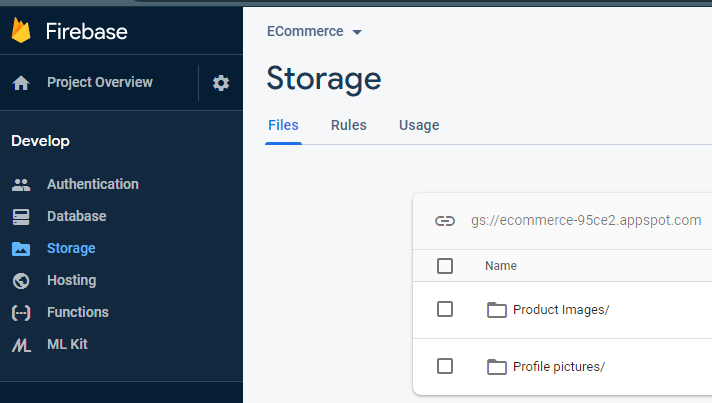
\includegraphics[width=0.45\textwidth]{Images/admin_products_storage_img.png}
	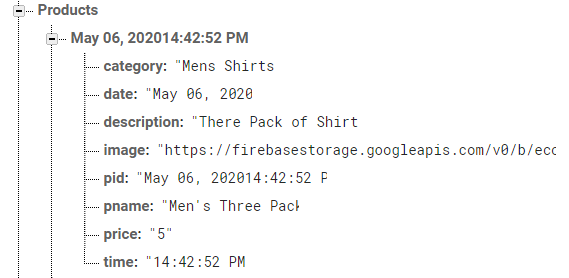
\includegraphics[width=0.45\textwidth]{Images/admin_products_storage_db.png}
\end{figure}
\newpage

\subsection{RecyclerView}
The RecyclerView is used to display all the products stored on the Database.
Implementation of this goes as follows:\newline

\textbf{1. Create the Product layout in a CardView, products\_layout\.xml}
\begin{figure}[h!]
	\caption{Product Layout and Design}
	\label{productlayout}
	\centering
	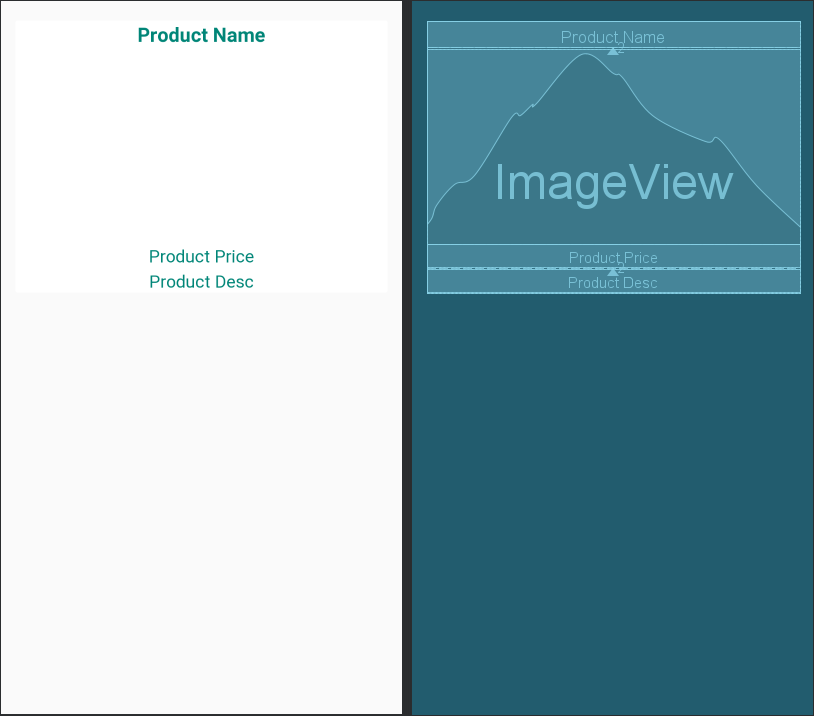
\includegraphics[width=0.6\textwidth]{Images/product_layout.png}
\end{figure}

\textbf{2. Create a Model Kotlin Class}
\begin{minted}{kotlin}
companion object{
    public lateinit var category:String
    public lateinit var date:String
    public lateinit var description:String
    public lateinit var image:String
    public lateinit var pid:String
    public lateinit var pname:String
    public lateinit var price:String
    public lateinit var time:String }
    
init {
        lateinit var category:String
        lateinit var date:String
        lateinit var description:String
        lateinit var image:String
        lateinit var pid:String
        lateinit var pname:String
        lateinit var price:String
        lateinit var time:String }
    
\end{minted}
\newpage
\textbf{3. Create a ProductViewHolder which implements ItemClickListener inferface}
\begin{minted}{kotlin}
class ProductView:RecyclerView.ViewHolder, View.OnClickListener{
    var txtProdName:TextView
    var txtProdDesc:TextView
    var txtProdPrice:TextView
    var txtImageView:ImageView
    lateinit var listener: ItemClickListener
    constructor(itemView: View) : super(itemView)

    fun ProductView(itemView:View){
        super.itemView
        txtImageView = itemView.findViewById(R.id.product_card_img)
        txtProdName = itemView.findViewById(R.id.product_card_name)
        txtProdDesc = itemView.findViewById(R.id.product_card_desc)
        txtProdPrice = itemView.findViewById(R.id.product_card_price)
    }

    init {
        txtImageView = itemView.findViewById(R.id.product_card_img)
        txtProdName = itemView.findViewById(R.id.product_card_name)
        txtProdDesc = itemView.findViewById(R.id.product_card_desc)
        txtProdPrice = itemView.findViewById(R.id.product_card_price)
    }

    fun setItemClickListener(listener: ItemClickListener){
        this.listener = listener
    }


    override fun onClick(v: View?) {
        listener.onClick(v!!, adapterPosition, false)
    }
}

\end{minted}

\textbf{4. Finally display the recyclerView in the HomeActivity}
\begin{minted}{kotlin}
override fun onStart() {
    super.onStart()

    val options = FirebaseRecyclerOptions.Builder<Products>().setQuery(productsRef, Products::class.java).build()

    val adapter:FirebaseRecyclerAdapter<Products, ProductView> = object:FirebaseRecyclerAdapter<Products, ProductView>(options) {
        override fun onBindViewHolder(holder: ProductView, position: Int, model: Products) {
            holder.txtProdName.setText(model.getPname())
            holder.txtProdDesc.setText(model.getDescription())
            holder.txtProdPrice.setText("Price: " + "€" + model.getPrice())       //"Price: ${price}$"
            Picasso.get().load(model.getImage()).into(holder.txtImageView)
        }

        override fun onCreateViewHolder(parent: ViewGroup, viewType: Int): ProductView {
            val view = LayoutInflater.from(parent.context).inflate(R.layout.products_layout, parent, false)
            return ProductView(view)
        }
    }//adapter
    recyclerView.adapter = adapter
    adapter.startListening()
}//onStart

\end{minted}

\begin{figure}[h!]
	\caption{Items displayed in RecyclerView}
	\label{productview}
	\centering
	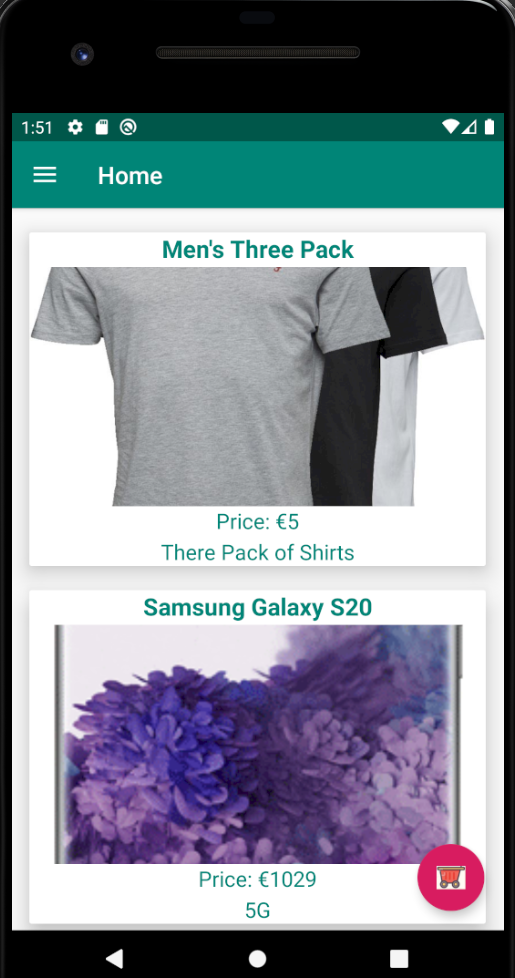
\includegraphics[width=0.5\textwidth]{Images/recycle_view_products.png}
\end{figure}
\newpage

\subsection{Settings}
The settings are used for the user to edit there User Profile details.
The user can choose a Profile image, as well as change there Phone Number, Name and Address

\begin{figure}[h!]
	\caption{View and Design - User Profile settings}
	\label{productview}
	\centering
	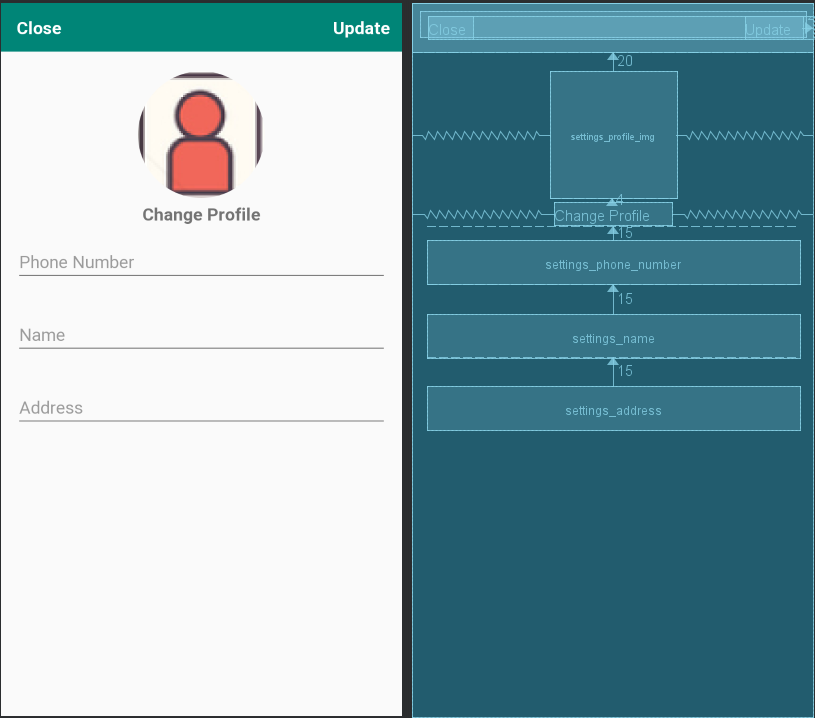
\includegraphics[width=0.8\textwidth]{Images/user_profile_settings_change.png}
\end{figure}

The code for settings is located in the SettingsFragment, this fragment contains three different aspects: Allowing User to choose a Profile Image, Saving the Users Details and Displaying Users New Details

\subsubsection{1. Allowing User to choose a Profile Image}
Once the user chooses to change there profile image a onClickListener will trigger to create the process
\begin{minted}{kotlin}
profileChangeTxtBtn.setOnClickListener{ it: View? ->
    check = "clicked"

    // for fragment (DO NOT use `getActivity()`)
    this.context?.let { it1 ->
        CropImage.activity()
            .setAspectRatio(1, 1)
            .start(it1, this)
\end{minted}

Once triggered this will prompt the User to choose a folder in there phone and contains the images they want to display as there profile picture. Once an image is chosen the user will be prompted with a screen to Crop that image 
\begin{figure}[h!]
	\caption{Crop image for User Profile Picture}
	\label{cropimg}
	\centering
	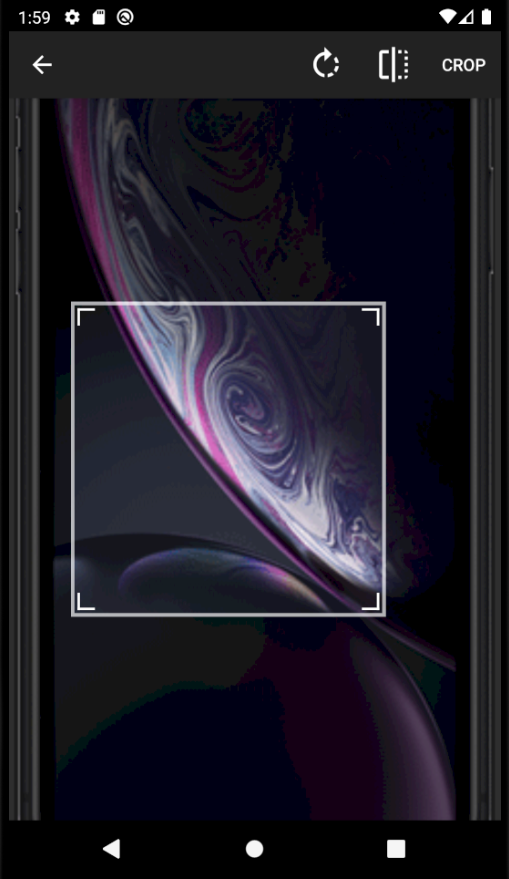
\includegraphics[width=0.6\textwidth]{Images/user_crop_img.png}
\end{figure}
\newpage
\subsubsection{Saving Cropped Image}
Once the User has chosen the cropped image that they like, a function onActivityResult will be called. This function will validate the cropped image as well as saving the image if it is suitable.

\begin{minted}{kotlin}
override fun onActivityResult(requestCode: Int, resultCode: Int, data: Intent?) {
    super.onActivityResult(requestCode, resultCode, data)

    if (requestCode == CropImage.CROP_IMAGE_ACTIVITY_REQUEST_CODE){
        val result = CropImage.getActivityResult(data)
        if (resultCode == RESULT_OK){
            imageUri = result.uri
            profileImageView.setImageURI(imageUri)
        }else if (resultCode == CropImage.CROP_IMAGE_ACTIVITY_RESULT_ERROR_CODE){
            var error = result.error
            Toast.makeText(this.context, "Error, please try again ", Toast.LENGTH_SHORT).show()
        }
    }
}
\end{minted}
\newpage

\subsubsection{2. Saving the Users Details}
There is two separate functions for saving the User Details. One function uploadImage() contains code for uploading the Cropped Image that the user has chosen to the Database and updateUserInfo() will update users data if they wish to not choose to upload a new profile picture.

\begin{figure}[h!]
	\caption{Update User Details}
	\label{userdetails}
	\centering
	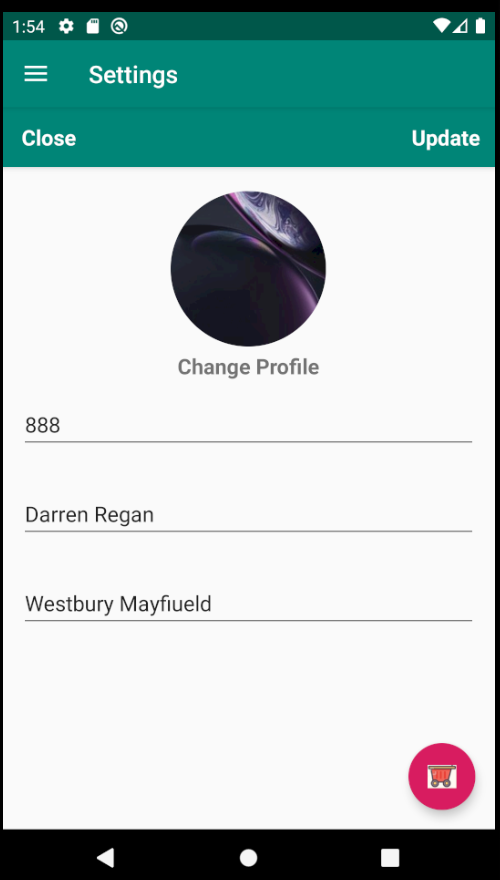
\includegraphics[width=0.6\textwidth]{Images/setting_updating.png}
\end{figure}
\newpage

\subsubsection{Updating all user details}
Once the user clicks the update button shown in Figure \ref{userdetails} it will trigger the onClickListener
\begin{minted}{kotlin}
saveTextBtn.setOnClickListener{ it: View? ->
    if (check == "clicked"){
        saveUserInfo()
    }
    else{
        updateUserInfo()
    }
}
\end{minted}

SaveUserInfo() is called when the user decides to upload a image, this will first validate that the user has entered details before calling the uploadImage() function

\begin{minted}{kotlin}
private fun saveUserInfo() {
    when {
        TextUtils.isEmpty(fullNameEditText.text.toString()) 
        -> Toast.makeText(this.context, "Must have a name ", Toast.LENGTH_SHORT).show()
        TextUtils.isEmpty(addressEditText.text.toString()) 
        -> Toast.makeText(this.context, "Must have a address ", Toast.LENGTH_SHORT).show()
        TextUtils.isEmpty(userPhoneEditText.text.toString()) 
        -> Toast.makeText(this.context, "Must have a phone number ", Toast.LENGTH_SHORT).show()
        check == "clicked" -> uploadImage()
    }
}
\end{minted}
\newpage
\subsubsection{Upload Image and Save Data}
Once triggered the process of saving the users detail will now start
\begin{minted}{kotlin}
run {
    val fileRef =
        storageProfilePicRef.child(Prevalent.currentOnlineUser.getPhone() + ".jpg")
    uploadTask = fileRef.putFile(imageUri)

    val ut = uploadTask.continueWithTask { task ->
        if (!task.isSuccessful) {
            task.exception?.let {
                throw it
            }
        }
        myUrl = fileRef.downloadUrl.toString()
        return@continueWithTask fileRef.downloadUrl
    }.addOnCompleteListener { task ->
        if (task.isSuccessful) {
            val downloadUrl = task.result
            myUrl = downloadUrl.toString()

            var ref = FirebaseDatabase.getInstance().reference.child("Users")
            var userMap:HashMap<String, Any> = HashMap()
            userMap["name"] = fullNameEditText.text.toString()
            userMap["address"] = addressEditText.text.toString()
            userMap["phoneOrder"] = userPhoneEditText.text.toString()
            //userMap["phone"] = userPhoneEditText.text.toString()
            userMap["image"] = myUrl
            ref.child(Prevalent.currentOnlineUser.getPhone()).updateChildren(userMap)

            progressDialog.dismiss()

            val intent = Intent(activity, HomeActivity::class.java)
            startActivity(intent)
            Toast.makeText(this.context, "Profile Updated! ", Toast.LENGTH_SHORT).show()
        }
      
\end{minted}
\newpage

\subsubsection{3. Display new User Details}
After saving all the details the User is sent to the HomeActivity, if user returns to the settings page there new details will be displayed shown in Figure \ref{userdetails}, the function displayUserInfo() is used to achieve this

\begin{minted}{kotlin}
private fun displayUserInfo(profileImageView: CircleImageView?, fullNameEditText: EditText?,
userPhoneEditText: EditText?, addressEditText: EditText?) {
    val usersRef = FirebaseDatabase.getInstance().reference.child("Users").child(Prevalent.currentOnlineUser.getPhone())

    usersRef.addValueEventListener(object: ValueEventListener {
        override fun onCancelled(p0: DatabaseError) {
        }

        override fun onDataChange(dataSnapshot: DataSnapshot) {
            if (dataSnapshot.exists()){
                if (dataSnapshot.child("image").exists()){
                    val image:String = dataSnapshot.child("image").value.toString()
                    val name:String = dataSnapshot.child("name").value.toString()
                    val phone:String = dataSnapshot.child("phone").value.toString()
                    val address:String = dataSnapshot.child("address").value.toString()

                    Picasso.get().load(image).into(profileImageView)
                    fullNameEditText?.setText(name)
                    userPhoneEditText?.setText(phone)
                    addressEditText?.setText(address)
                }
            }
        }
    })//EventListener
}//displayUserInfo
\end{minted}
\chapter{System Evaluation}


As many pages as needed.
• Prove that your software is robust. How? Testing etc.
• Use performance benchmarks (space and time) if algorithmic.
• Measure the outcomes / outputs of your system / software against the
objectives from the Introduction.
• Highlight any limitations or opportunities in your approach or technologies
used.

\section{Robust}
\subsection{Error Handling}
\subsection{Testing}
\subsection{Speed}

\section{Accessibility}
\subsection{Minimalistic}
\subsection{Intuitive}

\section{Evaluation of Objectives}
\subsection{Scalable}
\subsection{Can use as a template for any company}
\subsection{Responsive}
\subsection{Statistics}
talk about how firebase already has this built in and further coding was too advanced
\chapter{Conclusion}
This chapter serves as a conclusion to the project. In it, the objectives of the project are analysed again briefly to evaluate whether or not they were met. It also analyses any improvements and/or changes that could be added/made to the project if it was to be developed again.

\section{Objectives Review}
The overall rationale and goal for my project was i was considering Android Development as a career option and i wanted to gain experience in Native Development and developing with Native Tools such as Android Studio.\newline

\subsection{What i learned}
The main objectives for this project was to learn a new programming language and to learn and create a native android application. These two objectives are the most important as the main goal was to get insight on Android Development as Android Development was something i was debating on choosing as a main career option.
Through completing this Project i feel like i gained exactly what i wanted out of this project and i am now highly considering Android Development as my career going forward. 
\bigskip

\section{Improvements}
There are many improvements i would want to make to my application, integrating the many products from Firebase shown in the tech review, creating a product analysis, creating consumer statistics for buying habits, integrating Google Analytics for advertisements etc. All of these we're considered and even attempted but were ultimately out of scope of a non-team project.
\bigskip

\section{Downfalls}
These are some downfalls of the project, i give my thoughts on what i learned and how i would fix these issues going forward. These two i feel like are actually a huge benefit for me to have a downfall on before i go into industry. I know of these problems from our study but have never actually experienced them properly, this experience should give me insight before going into industry on how i should plan out my work and how valuable Software Methodologies such as Agile are to developing software.

\subsection{Scope Creep}
Scope creep was hard to manage in this project as i kept wanting to add more features before i had a solid foundation. I originally wanted an employee chat and calendar to manage work days, additionally i wanted to add statistics for purchasing habits etc. But all these features made no sense in the scope of this project as i am solo. If i had two addition persons then these features would be feasible, but i wasted a good amount of time researching how i would develop these features instead of just coding the more basic features of the project.

Scope Creep had a very negative impact on this project for this reason, and is something i have learned a great deal amount now that i have actually experienced it.\newline

\textbf{Ways i found to combat scope-creep}:
\begin{itemize}
    \item \textbf{Planning}- Carefully planning out the features/components and sticking to that plan and only branching out when the plan is complete or is needed. This would make it less likely to fall prey to scope-creep
    \item \textbf{Focus on Main Features} - Focusing on the main features that i had described in my deign document is the easiest way to combat scope-creep. I had laid out features but over time i focused less and less on those features and branched off to area's and didn't add anything to the actual project.
    
    After this project i now know a lot more on how to focus on the important features, making sure they're implemented and tested adequately before implementing new features.
    \item \textbf{Utilizing Development Cycles} - I feel like i should have utilized Test driven development more, i believe i should of just implemented the feature and gone back to refactor it to save a lot of time. But i mostly ended up not implementing a lot of stuff due to time constraints.
\end{itemize}

\subsection{Utilize Docs}
What i noticed with Kotlin and Android Development, is that there is a huge amount of documentation that i didn't end up reading, so i would implement for example Firebase authentication and Login/Sign-up features through trial and error. But there was a resource available for it for free which i previously thought cost a fixed amount.
So what i learned is that reading the full documentation is a huge benefit before trying to implement a feature.
Documentation for Android, not only helps with implementing features but also have a large amount of tips on UI Design, Marketing Strategies, Performance Tips and many more topics. 

\bigskip

\section{System Evaluation}
highlight findings from, system evaluation

List out the outcomes of the project in a bulleted list.
– Serendipity – did you gain any tangential or even unrelated insights
by happen chance during the project?
• Lots of discoveries have been made this way, e.g. Flemming
and antibiotics.
– State any opportunities identified for future investigation.
\bigskip

\section{Final Conclusion}
This project was a great learning experience. It has given me real insight on how important actual Software Methodologies are to creating Software in a timely manner. I gained experience with a new language and development platform as well. I am actually interested in Android Development as a career after working with Android Studio and Kotlin. The project as a whole just highlights the benefit of Software Development Methodologies and their usage within Industry. Time management is also something highlighted as it played a large role and shows just how important deadlines are within companies. This project provided great experience and knowledge that i know will help me within industry in the future.\newline

As a Final Word, i would like to extend my thanks and gratitude to all of the lecturers at GMIT who have helped me in various ways throughout the last four years. It is thanks to the staff at GMIT that i can go forward into industry with a positive mindset and the ability to learn and adapt to what the industry requires of me. Finally i would like to thank my personal supervisor Martin Hynes and the external examiners who will be grading this project, i hope you find the documentation and code to be of rigorous academic standards.
\bigskip
\chapter{Appendices}

\subsubsection{Github Repository}
\url{https://github.com/DarrenRegan/Final-Year-Project}

\subsubsection{Github Kanban Board}
\url{https://github.com/DarrenRegan/Final-Year-Project/projects/1}

\subsubsection{Github Kotlin Code}
\url{https://github.com/DarrenRegan/Final-Year-Project/tree/master/app/src/main/java/com/example/ecommerce}

\subsubsection{Github XML Files}
\url{https://github.com/DarrenRegan/Final-Year-Project/tree/master/app/src/main/res/layout}

\subsubsection{Screencast}
\url{https://youtu.be/lY1Y_oAYKdc}






%----------------------------------------------------------------------------------------
%   5) REFERENCES
%      create ref in references.bib and \cite here
%----------------------------------------------------------------------------------------
\printbibliography[title={References}]
\cite{firebase_products}
\cite{firebase}
\cite{salesforce_native_hyrbid}
\cite{react_native_ex10}
\cite{react_native_ex20}
\cite{android_perf_tips}
\cite{firebase_docs}
\cite{firebase_docs_auth}
\cite{firebase_docs_realtimedb}
\cite{firebase_docs_storage}
\cite{phone_market_share}
\cite{codelab_android}
\cite{firebase_pricing}
\cite{picasso_github}
\cite{badges}
\cite{FDD}
\cite{FDD_paper1}
\cite{docu_article1}
\cite{Cont_delivery_1}
\cite{Cont_delivery_2}
\cite{android_key_sign}
\cite{cd_gitlab}
\cite{cd_circleci}
\cite{cd_codeship}
\cite{cd_github}
\cite{cd_aws}
\cite{mob_app_paper_challenges}
\cite{mvp_paper}
\cite{ionic_hybid_app}
\cite{cordova_hybid_app}
\cite{ionic_hybrid_roi}
\cite{android_sup_java}
\cite{android_single_activity_summitvid}
\cite{android_single_activity_blog}
\cite{android_activity_docs}
\cite{android_activity_fragments}
\cite{android_guide_arc}
\cite{paper}
\cite{android_jetpack}
\cite{android_lifecycles}
\end{document}